\chapter{Funções}

\section{Definição de funções}

\vskip0.3cm
 \colorbox{azul}{
 \begin{minipage}{0.9\linewidth}
 \begin{center}
  Dados dois conjuntos $A$ e $B$ não vazios, de números Reais, ou seja, $A \subseteq \mathbb{R}$ e $B \subseteq \mathbb{R}$. Uma \textbf{aplicação} de $A$ em $B$ ou \textbf{função} definida no conjunto $A$ com imagens em $B$ é uma regra (equação) que diz como associar cada elemento $x \in A$ a um \underline{único} $y \in B$.
 \end{center}
 \end{minipage}}
 \vskip0.3cm


 Exemplos de relações que são funções de $A$ em $B$:
 \begin{multicols}{3}
 \begin{tikzpicture}
 \node (1) at (0,0) {1};%\filldraw(1.east) circle (1pt)
 \node (2) [below of=1] {2};%\filldraw(2.east) circle (1pt)
 \node (3) [below of=2] {3};%\filldraw(3.east) circle (1pt)
 \node[fit=(1) (2) (3),ellipse,draw=red,minimum width=1cm,thick,label=below:\(A\)]{};

 \node (a) at (3,0) {a};%\filldraw($b_1$.west) circle (1pt)
 \node (b) [below of=a] {b};%\filldraw($b_2$.west) circle (1pt)
 \node (c) [below of=b] {c};%\filldraw($b_3$.west) circle (1pt)
 \node[fit=(a) (b) (c),ellipse,draw=green,minimum width=1cm,thick,label=below:\(B\)]{};

 \draw[->, shorten >=.1cm, >=stealth'] (1.east) to (a.west);
 \draw[->, shorten >=.1cm, >=stealth'] (2.east) to (b.west);
 \draw[->, shorten >=.1cm, >=stealth'] (3.east) to (c.west);
\end{tikzpicture} \\
 \begin{tikzpicture}
 \node (1) at (0,0) {1};%\filldraw(1.east) circle (1pt)
 \node (2) [below of=1] {2};%\filldraw(2.east) circle (1pt)
 \node (3) [below of=2] {3};%\filldraw(3.east) circle (1pt)
 \node[fit=(1) (2) (3),ellipse,draw=red,minimum width=1cm,thick,label=below:\(A\)]{};

 \node (a) at (3,0) {a};%\filldraw($b_1$.west) circle (1pt)
 \node (b) [below of=a] {b};%\filldraw($b_2$.west) circle (1pt)
 \node (c) [below of=b] {c};%\filldraw($b_3$.west) circle (1pt)
 \node[fit=(a) (b) (c),ellipse,draw=green,minimum width=1cm,thick,label=below:\(B\)]{};

 \draw[->, shorten >=.1cm, >=stealth'] (1.east) to (a.west);
 \draw[->, shorten >=.1cm, >=stealth'] (2.east) to (a.west);
 \draw[->, shorten >=.1cm, >=stealth'] (3.east) to (c.west);
\end{tikzpicture} \\
\begin{tikzpicture}
 \node (1) at (0,0) {1};%\filldraw(1.east) circle (1pt)
 \node (2) [below of=1] {2};%\filldraw(2.east) circle (1pt)
 \node (3) [below of=2] {3};%\filldraw(3.east) circle (1pt)
 \node[fit=(1) (2) (3),ellipse,draw=red,minimum width=1cm,thick,label=below:\(A\)]{};

 \node (a) at (3,0) {a};%\filldraw($b_1$.west) circle (1pt)
 \node (b) [below of=a] {b};%\filldraw($b_2$.west) circle (1pt)
 \node (c) [below of=b] {c};%\filldraw($b_3$.west) circle (1pt)
 \node[fit=(a) (b) (c),ellipse,draw=green,minimum width=1cm,thick,label=below:\(B\)]{};

 \draw[->, shorten >=.1cm, >=stealth'] (1.east) to (b.west);
 \draw[->, shorten >=.1cm, >=stealth'] (2.east) to (b.west);
 \draw[->, shorten >=.1cm, >=stealth'] (3.east) to (b.west);
\end{tikzpicture}

\end{multicols}



 Exemplos de relações que não são funções de $A$ em $B$:
\begin{multicols}{3}
\begin{tikzpicture}
 \node (1) at (0,0) {1};%\filldraw(1.east) circle (1pt)
 \node (2) [below of=1] {2};%\filldraw(2.east) circle (1pt)
 \node (3) [below of=2] {3};%\filldraw(3.east) circle (1pt)
 \node[fit=(1) (2) (3),ellipse,draw=red,minimum width=1cm,thick,label=below:\(A\)]{};

 \node (a) at (3,0) {a};%\filldraw($b_1$.west) circle (1pt)
 \node (b) [below of=a] {b};%\filldraw($b_2$.west) circle (1pt)
 \node (c) [below of=b] {c};%\filldraw($b_3$.west) circle (1pt)
 \node[fit=(a) (b) (c),ellipse,draw=green,minimum width=1cm,thick,label=below:\(B\)]{};

 \draw[->, shorten >=.1cm, >=stealth'] (1.east) to (a.west);
 \draw[->, shorten >=.1cm, >=stealth'] (1.east) to (b.west);
 \draw[->, shorten >=.1cm, >=stealth'] (2.east) to (b.west);
 \draw[->, shorten >=.1cm, >=stealth'] (3.east) to (c.west);
\end{tikzpicture} \\
\begin{tikzpicture}
 \node (1) at (0,0) {1};%\filldraw(1.east) circle (1pt)
 \node (2) [below of=1] {2};%\filldraw(2.east) circle (1pt)
 \node (3) [below of=2] {3};%\filldraw(3.east) circle (1pt)
 \node[fit=(1) (2) (3),ellipse,draw=red,minimum width=1cm,thick,label=below:\(A\)]{};

 \node (a) at (3,0) {a};%\filldraw($b_1$.west) circle (1pt)
 \node (b) [below of=a] {b};%\filldraw($b_2$.west) circle (1pt)
 \node (c) [below of=b] {c};%\filldraw($b_3$.west) circle (1pt)
 \node[fit=(a) (b) (c),ellipse,draw=green,minimum width=1cm,thick,label=below:\(B\)]{};

 \draw[->, shorten >=.1cm, >=stealth'] (1.east) to (a.west);
 %\draw[->, shorten >=.1cm, >=stealth'] (2.east) to (b.west);
 \draw[->, shorten >=.1cm, >=stealth'] (3.east) to (c.west);
\end{tikzpicture} \\
\begin{tikzpicture}
 \node (1) at (0,0) {1};%\filldraw(1.east) circle (1pt)
 \node (2) [below of=1] {2};%\filldraw(2.east) circle (1pt)
 \node (3) [below of=2] {3};%\filldraw(3.east) circle (1pt)
 \node[fit=(1) (2) (3),ellipse,draw=red,minimum width=1cm,thick,label=below:\(A\)]{};

 \node (a) at (3,0) {a};%\filldraw($b_1$.west) circle (1pt)
 \node (b) [below of=a] {b};%\filldraw($b_2$.west) circle (1pt)
 \node (c) [below of=b] {c};%\filldraw($b_3$.west) circle (1pt)
 \node[fit=(a) (b) (c),ellipse,draw=green,minimum width=1cm,thick,label=below:\(B\)]{};

 \draw[->, shorten >=.1cm, >=stealth'] (1.east) to (a.west);
 \draw[->, shorten >=.1cm, >=stealth'] (1.east) to (b.west);
 %\draw[->, shorten >=.1cm, >=stealth'] (2.east) to (b.west);
 \draw[->, shorten >=.1cm, >=stealth'] (3.east) to (c.west);
\end{tikzpicture}
\end{multicols}

\newpage

Usamos normalmente a seguinte notação:
\[f: A \rightarrow B\]
que se lê: $f$ é uma função de $A$ em $B$.

A função $f$ transforma $x \in A$ em $y \in B$. Denotamos isso da seguinte forma:
\[f(x) = y .\]

Simplificando as notações podemos representar as duas informações acima da seguinte forma:
\begin{eqnarray*}
 f: A & \rightarrow & B \\
 x & \mapsto & y.
\end{eqnarray*}

Dada uma função $f: A \rightarrow B$, o conjunto $A$ chama-se \textbf{domínio} da função $f$ e o conjunto $B$ chama-se \textbf{contradomínio} da função $f$.  Para cada $x \in A$, o elemento $f(x)= y \in B$ chama-se imagem de $x$ pela função $f$. Assim o conjunto \textbf{imagem} da função $f$ é dado por:
\[Im(f)= \{ y \in B \mid y = f(x) \text{ para algum } x \in A\} .\]

No nosso contexto, o domínio de uma função é um subconjunto dos números Reais nos quais faz sentido aplicar a regra da função, e o contradomínio é o conjunto $\mathbb{R}$, ou um subconjunto de $\mathbb{R}$ que contenha o conjunto $Im(f)$.

E o \textbf{gráfico} da função é dado por:
\[Gr(f) = \{ (x, y) \in A \times B \mid x \in A, y = f(x) \in B\} .\]

\begin{exem}
 Considere os conjuntos $A= \{1, 2, 3\}$ e $B= \{a, b, c, d\}$ e a regra de relação entre estes dois conjuntos dada pelo diagrama abaixo:

 \begin{figure}[H]
 \centering
 \begin{tikzpicture}
 \node (1) at (0,0) {1};%\filldraw(1.east) circle (1pt)
 \node (2) [below of=1] {2};%\filldraw(2.east) circle (1pt)
 \node (3) [below of=2] {3};%\filldraw(3.east) circle (1pt)
 \node[fit=(1) (2) (3),ellipse,draw=red,minimum width=1cm,thick,label=below:\(A\)]{};

 \node (a) at (3,0) {a};%\filldraw($b_1$.west) circle (1pt)
 \node (b) [below of=a] {b};%\filldraw($b_2$.west) circle (1pt)
 \node (c) [below of=b] {c};%\filldraw($b_3$.west) circle (1pt)
 \node (d) [below of=c] {d};%\filldraw($b_3$.west) circle (1pt)
 \node[fit=(a) (b) (c) (d),ellipse,draw=green,minimum width=1cm,thick,label=below:\(B\)]{};

 \draw[->, shorten >=.1cm, >=stealth'] (1.east) to (b.west);
 \draw[->, shorten >=.1cm, >=stealth'] (2.east) to (c.west);
 \draw[->, shorten >=.1cm, >=stealth'] (3.east) to (a.west);
\end{tikzpicture}
\end{figure}

Note que esta regra define uma função $f: A \rightarrow B$, cujo domínio é $Dom(f) = A$, contra-domínio é $CDom(f) = B$, e a imagem é $Im(f)= \{a, b, c\}$, observe que $Im(f) \subset CDom(f)$. Pela definição, temos que o gráfico da $f$ será o conjunto
\[
Gr(f)= \{(1, b); (2, c); (3, a)\}
\]
que pode ser representado geometricamente como feito na figura abaixo:

\begin{figure}[H]
 \centering
    \fbox{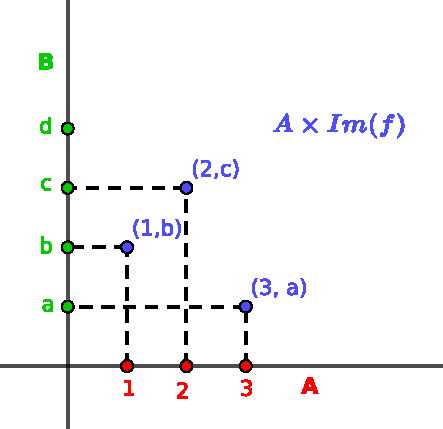
\includegraphics[width=7cm]{../Topicos/Figuras/Grf.pdf}}
    \caption{Gráfico da função $f$}
  \end{figure}

\end{exem}


\subsection{Propriedades}
As funções são classificadas em:

\begin{itemize}
 \item \textbf{Injetora}

 Uma função $f: A \rightarrow B$ é injetiva, ou injetora quando:
 \[ x_1 \neq x_2 \in A \Rightarrow f(x_1) \neq f(x_2) \in B ,\]
 ou equivalentemente usando a contrapositiva:
 \[f(x_1) = f(x_2) \in B \Rightarrow x_1 = x_2 .\]
 Ou seja, quando cada elemento da $Im(f)$ recebe um único elemento de $A= Dom(f)$, neste caso pode ocorrer de alguns elementos de $B$ não serem imagem de nenhum elemento de $A$ pela função $f$.

 \item \textbf{Sobrejetora}

 Uma função $f: A \rightarrow B$ é sobrejetiva, ou sobrejetora quando para todo $y \in B$, existe pelo menos um elemento $x \in A$ tal que $f(x) = y$. Equivalentemente em símbolos:
 $$\forall y \in B, \exists x \in A \text{ tal que } f(x) = y$$
 Ou ainda, quando cada elemento de $B$ recebe algum elemento de $A$, neste caso podendo não ser único.

 \item \textbf{Bijetora}

 Uma função $f: A \rightarrow B$ é bijetora, ou bijetiva quando for simultaneamente injetora e sobrejetora. Neste caso, $f$ admite uma inversa que é denotada por $f^{(-1)}$.

\end{itemize}

\begin{multicols}{2}
 \begin{tikzpicture}
 \node (1) at (0,0) {1};%\filldraw(1.east) circle (1pt)
 \node (2) [below of=1] {2};%\filldraw(2.east) circle (1pt)
 \node (3) [below of=2] {3};%\filldraw(3.east) circle (1pt)
 \node[fit=(1) (2) (3),ellipse,draw=red,minimum width=1cm,thick,label=below:\(A\)]{};

 \node (a) at (3,0) {a};%\filldraw($b_1$.west) circle (1pt)
 \node (b) [below of=a] {b};%\filldraw($b_2$.west) circle (1pt)
 \node (c) [below of=b] {c};%\filldraw($b_3$.west) circle (1pt)
 \node[fit=(a) (b) (c),ellipse,draw=green,minimum width=1cm,thick,label=below:\(B\)]{};

 \draw[->, shorten >=.1cm, >=stealth'] (1.east) to (c.west);
 \draw[->, shorten >=.1cm, >=stealth'] (2.east) to (b.west);
 \draw[->, shorten >=.1cm, >=stealth'] (3.east) to (a.west);
\end{tikzpicture} \\
 \textbf{bijetora}\\
 \begin{tikzpicture}
 \node (1) at (0,0) {1};%\filldraw(1.east) circle (1pt)
 \node (2) [below of=1] {2};%\filldraw(2.east) circle (1pt)
 \node (3) [below of=2] {3};%\filldraw(3.east) circle (1pt)
 \node[fit=(1) (2) (3),ellipse,draw=red,minimum width=1cm,thick,label=below:\(A\)]{};

 \node (a) at (3,0) {a};%\filldraw($b_1$.west) circle (1pt)
 \node (b) [below of=a] {b};%\filldraw($b_2$.west) circle (1pt)
 \node[fit=(a) (b),ellipse,draw=green,minimum width=1cm,thick,label=below:\(B\)]{};

 \draw[->, shorten >=.1cm, >=stealth'] (1.east) to (a.west);
 \draw[->, shorten >=.1cm, >=stealth'] (2.east) to (a.west);
 \draw[->, shorten >=.1cm, >=stealth'] (3.east) to (b.west);
\end{tikzpicture} \\
\textbf{sobrejetora e não injetora}
\end{multicols}

\begin{multicols}{2}
 \begin{tikzpicture}
 \node (1) at (0,0) {1};%\filldraw(1.east) circle (1pt)
 \node (2) [below of=1] {2};%\filldraw(2.east) circle (1pt)
 \node (3) [below of=2] {3};%\filldraw(3.east) circle (1pt)
 \node[fit=(1) (2) (3),ellipse,draw=red,minimum width=1cm,thick,label=below:\(A\)]{};

 \node (a) at (3,0) {a};%\filldraw($b_1$.west) circle (1pt)
 \node (b) [below of=a] {b};%\filldraw($b_2$.west) circle (1pt)
 \node (c) [below of=b] {c};%\filldraw($b_3$.west) circle (1pt)
 \node[fit=(a) (b) (c),ellipse,draw=green,minimum width=1cm,thick,label=below:\(B\)]{};

 \draw[->, shorten >=.1cm, >=stealth'] (1.east) to (b.west);
 \draw[->, shorten >=.1cm, >=stealth'] (2.east) to (b.west);
 \draw[->, shorten >=.1cm, >=stealth'] (3.east) to (a.west);
\end{tikzpicture} \\
\textbf{não sobrejetora e não injetora}\\
 \begin{tikzpicture}
 \node (1) at (0,0) {1};%\filldraw(1.east) circle (1pt)
 \node (2) [below of=1] {2};%\filldraw(2.east) circle (1pt)
 \node (3) [below of=2] {3};%\filldraw(3.east) circle (1pt)
 \node[fit=(1) (2) (3),ellipse,draw=red,minimum width=1cm,thick,label=below:\(A\)]{};

 \node (a) at (3,0) {a};%\filldraw($b_1$.west) circle (1pt)
 \node (b) [below of=a] {b};%\filldraw($b_2$.west) circle (1pt)
 \node (c) [below of=b] {c};%\filldraw($b_3$.west) circle (1pt)
 \node (d) [below of=c] {d};%\filldraw($b_3$.west) circle (1pt)
 \node[fit=(a) (b) (c) (d),ellipse,draw=green,minimum width=1cm,thick,label=below:\(B\)]{};

 \draw[->, shorten >=.1cm, >=stealth'] (1.east) to (b.west);
 \draw[->, shorten >=.1cm, >=stealth'] (2.east) to (c.west);
 \draw[->, shorten >=.1cm, >=stealth'] (3.east) to (a.west);
\end{tikzpicture} \\
\textbf{não sobrejetora e injetora}
\end{multicols}

\begin{exem}

 \begin{enumerate}
  \item $f: \mathbb{R} \rightarrow \mathbb{R}$ tal que $f(x) = x^2$

  Neste caso, $f$ não é sobrejetora, nem injetora.

  \begin{dem}

   \begin{itemize}
    \item Sobrejetora

    $f$ não é sobrejetora porque $x^2 \geq 0$, $\forall x \in \mathbb{R}$, logo se considerarmos $y < 0 \in \mathbb{R}$ teremos que $\nexists x \in \mathbb{R}$ tal que $f(x)= y$. Portanto $f$ não é sobrejetora.
    \fim
    \item Injetora

     Note que $ \forall x \in \mathbb{R} \Rightarrow -x \in \mathbb{R}$ e que
    \[f(-x)= (-x)^2 = (-x)*(-x) = (x)*(x) = x^2 = f(x)\]
    o que mostra que $f$ não é injetora.

   \end{itemize}
  \end{dem}

  \item $f: \mathbb{R_{+}} \rightarrow \mathbb{R}$ tal que $f(x) = x^2$

  Neste caso, $f$ não é sobrejetora, mas é injetora.

  \begin{dem}
   \begin{itemize}
    \item Sobrejetora

    $f$ não é sobrejetora porque $x^2 \geq 0$, $\forall x \in \mathbb{R}$, logo se considerarmos $y < 0 \in \mathbb{R}$ teremos que $\nexists x \in \mathbb{R}$ tal que $f(x)= y$. Portanto $f$ não é sobrejetora.
    \fim
    \item Injetora

    Tome $x_1=x_2 \in \mathbb{R_{+}}$ qualquer, como
    \[x_1=x_2 \Rightarrow x_1^2=x_2^2 \Rightarrow f(x_1)=f(x_2)\]
    logo $f$ é injetora.

   \end{itemize}
  \end{dem}

  \item $f: \mathbb{R} \rightarrow \mathbb{R_{+}}$ tal que $f(x) = x^2$

  Neste caso, $f$ é sobrejetora, mas não é injetora.

  \begin{dem}
   \begin{itemize}
    \item Sobrejetora

    Tome $y \in \mathbb{R_{+}}$ qualquer, como $y \geq 0$ existe $x \in \mathbb{R}$ tal que
    \[x = \sqrt{y} \Rightarrow x^2 = (\sqrt{y})^2 \Rightarrow x^2 = y \Rightarrow f(x) = y \]
    portanto $f$ é sobrejetora.
    \fim
    \item Injetora

    Note que $ \forall x \in \mathbb{R} \Rightarrow -x \in \mathbb{R}$ e que
    \[f(-x)= (-x)^2 = (-x)*(-x) = (x)*(x) = x^2 = f(x)\]
    o que mostra que $f$ não é injetora.

   \end{itemize}
  \end{dem}

  \item $f: \mathbb{R_{+}} \rightarrow \mathbb{R_{+}}$ tal que $f(x) = x^2$ ou $f: \mathbb{R_{-}} \rightarrow \mathbb{R_{+}}$ tal que $f(x) = x^2$

  Neste caso, $f$ é sobrejetora, e é injetora, portanto bijetora.

  \begin{dem}
   \begin{itemize}
    \item Sobrejetora

    Tome $y \in \mathbb{R_{+}}$ qualquer, como $y \geq 0$ existe $x \in \mathbb{R}$ tal que
    \[x = \sqrt{y} \Rightarrow x^2 = (\sqrt{y})^2 \Rightarrow x^2 = y \Rightarrow f(x) = y\]
    portanto $f$ é sobrejetora.
    \fim
    \item Injetora

    Tome $x_1, x_2 \in \R_{+}$, tais que $f(x_1) = f(x_2)$ logo,
    \[f(x_1) = f(x_2) \Rightarrow x_1^2= x_2^2 \Rightarrow \sqrt{x_1^2}= \sqrt{x_2^2} \Rightarrow |x_1|= |x_2| \Rightarrow x_1= x_2, \]
    pois $x_1, x_2 \geqslant 0$. Portanto $f$ é injetora.

   \end{itemize}
  \end{dem}

 \end{enumerate}

\end{exem}

\subsection{Operações com funções}
Dadas as funções $f: A \rightarrow \R$, $g: B \rightarrow \R$, se $A \cap B \neq \emptyset$, então $\forall x \in A \cap B$, definimos as seguintes operações entre estas funções:
\[(f + g)(x)= f(x) + g(x); \]
\[(f - g)(x)= f(x) - g(x); \]
\[(f \cdot g)(x)= f(x) \cdot g(x); \]
\[ \left( \frac{f}{g} \right) (x)= \frac{f(x)}{g(x)} ;\]
\[(k \cdot f)(x)= k \cdot f(x), \text{ para } k \text{ constante} ,\]

note que:
\[dom(f+g)= dom(f-g)= dom(f \cdot g)= dom(k \cdot f)= A \cap B ,\]
\[ dom\left( \frac{f}{g} \right)= \{x \in A \cap B \mid g(x) \neq 0\}. \]

Além destas operações, é possível também definir a composição de funções. Para isso consideremos duas funções $f: A \rightarrow B$ e $g: C \rightarrow D$, com $A, B, C \text{ e } D \subset \R$, e tais que $Im(f) \subset C$ , assim a função composta $g \circ f: A \rightarrow D$ é definida por:
\[(g \circ f)(x)= g(f(x)). \]

\section{Tipos de funções}

\subsection{Função constante}

É a função que associa todos os elementos do domínio a um único elemento do contradomínio. Ou seja, dado $a \in \R$ fixo, a função $f$:
\begin{eqnarray*}
 f: \R & \rightarrow & \R \\
 x & \mapsto & a,
\end{eqnarray*}
é uma função constante.

Por exemplo, a função $f$:
\begin{eqnarray*}
 f: \R & \rightarrow & \R \\
 x & \mapsto & 2 \ .
\end{eqnarray*}

É uma função constante. Para construir o gráfico desta função começamos encontrando alguns pontos $(x, y)= (x, f(x))$ do gráfico, o que pode ser feito através da seguinte tabela:

 \begin{table}[H]
 \centering
 \begin{tabular}{|c|c|c|} \hline
 \rowcolor{cinza}
  x & f(x)= 2 & (x, y)  \\\hline
  -1 & f(-1)= 2 & (-1, 2) \\\hline
   0 & f(0)= 2 & (0, 2)  \\\hline
   1 & f(1)= 2 & (1, 2) \\\hline
 \end{tabular}
\end{table}

Após encontrar os pontos basta marcar os mesmo o plano cartesiano e traçar a curva que liga estes pontos com isso objetos o gráfico da função. Neste caso o gráfico é:
\begin{figure}[H]
 \centering
    \fbox{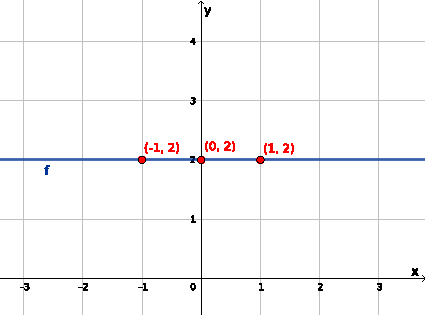
\includegraphics[width=7cm]{../Topicos/Figuras/f(x)=2.pdf}}
    \caption{Gráfico da função $f(x)=2$}
  \end{figure}

\subsection{Função identidade}

A função $Id$:
\begin{eqnarray*}
 Id: \R & \rightarrow & \R \\
 x & \mapsto & x \ ,
\end{eqnarray*}
é chamada \textit{função identidade real}.

Para encontrar alguns pontos $(x, f(x))$ do gráfico desta função, construímos a seguinte tabela:

 \begin{table}[H]
 \centering
 \begin{tabular}{|c|c|c|} \hline
 \rowcolor{cinza}
  x & f(x)= x & (x, y)  \\\hline
  -1 & f(-1)= -1 & (-1, -1) \\\hline
   0 & f(0)= 0 & (0, 0)  \\\hline
   1 & f(1)= 1 & (1, 1) \\\hline
 \end{tabular}
\end{table}

Logo o gráfico da função $Id$ é:
\begin{figure}[H]
 \centering
    \fbox{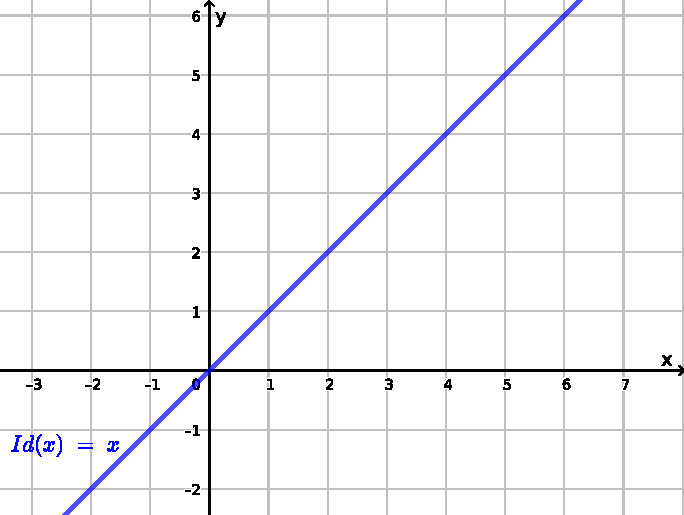
\includegraphics[width=7cm]{../Topicos/Figuras/Id(x)=x.pdf}}
    \caption{Gráfico da função $Id(x)=x$}
  \end{figure}


\subsection{Funções polinomiais de grau \texorpdfstring{$n$}{n}}

 \vskip0.3cm
 \colorbox{azul}{
 \begin{minipage}{0.9\linewidth}
 \begin{center}
 As funções $f: \R \to \R$ com a seguinte regra geral:
 \[f(x) = a_0 + a_1 x + a_2 x^2 + a_3 x^3 + \cdots + a_n x^n\]
 para $\{a_0, a_1, a_2, a_3, \ldots a_n\} \in \R$ e $n \in \N$, tais que $a_n \neq 0$ são denominadas \\ \textbf{funções polinomiais de grau $n$}.
 \end{center}
 \end{minipage}}
 \vskip0.3cm

 

 Casos particulares:
 \begin{itemize}
 \item Funções do 1º grau, ou funções afim

 São funções $f: \R \rightarrow \R$ dadas por:
 \[f(x)= ax + b \ , \]

 para certos $a, b \in \R$ com $a \neq 0$. Note que um caso particular e já conhecido de função de 1º grau é a função identidade, $f(x)= x$, a qual possui $a=1$ e $b=0$. 
 
 Vejamos mais alguns exemplos de funções de 1º grau.
 
 Consideremos as funções $f, g: \R \to \R$ dadas por:
 \begin{enumerate}[a)]
  \item $f(x)= x+2$
  \item $g(x)= x-1$
 \end{enumerate}

 
 \begin{figure}[H]
   \fbox{\subfigure[$f(x)= x+2$]{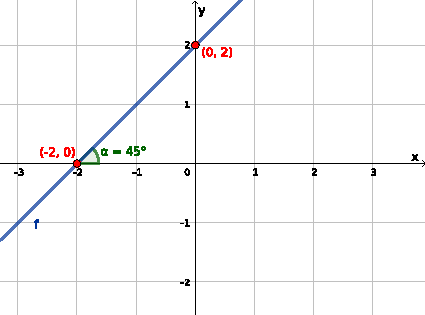
\includegraphics[width=7cm,height=6cm]{../Topicos/Figuras/f(x)=x+2.pdf}}}
   \fbox{\subfigure[$g(x)= x-1$]{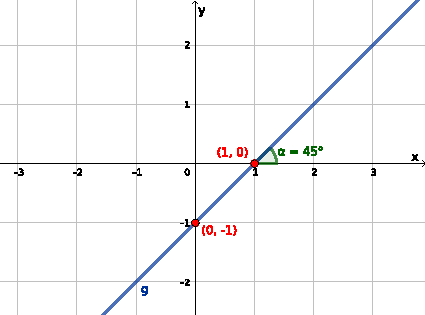
\includegraphics[width=7cm,height=6cm]{../Topicos/Figuras/f(x)=x-1.pdf}}}
  \end{figure} 
  Note que o que muda na definição destas funções é apenas o coeficiente $b$. Fazendo uma análise comparativa dos gráficos destas funções notamos que os ângulos que as retas formam com o eixo $x$ é o mesmo, portanto as retas são paralelas, porém o ponto de interseção das retas com o eixo $y$, que são os pontos $(0, f(0))$, $(0, g(0))$ muda, ou seja, $f(0) \neq g(0)$. De fato:
  \[f(0)= 0 + 2= 2\]
  \[g(0)= 0 -1 = -1 \ .\]
  No caso geral em que $f(x)=ax+b$, teremos que $f(0)=a0 + b= b$, portanto o gráfico de $f$ irá intersectar o eixo $y$ no ponto $(0,b)$. O coeficiente $b$ é chamado de \textbf{coeficiente linear} da reta/função linear.
  
  Consideremos as funções $f, g: \R \to \R$ dadas por:
 \begin{enumerate}[a)]
  \item $f(x)= 2x$
  \item $g(x)= -2x$
 \end{enumerate}
  
 \begin{figure}[H]
   \fbox{\subfigure[$f(x)= 2x$]{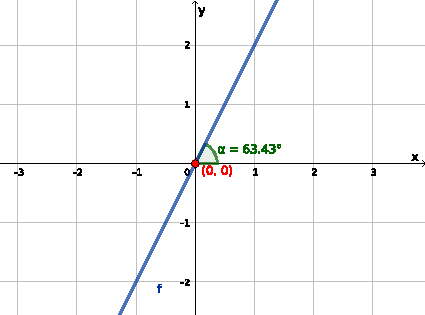
\includegraphics[width=7cm,height=6cm]{../Topicos/Figuras/f(x)=2x.pdf}}}
   \fbox{\subfigure[$g(x)= -2x$]{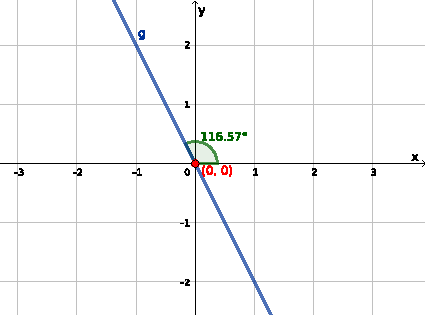
\includegraphics[width=7cm,height=6cm]{../Topicos/Figuras/g(x)=-2x.pdf}}}
  \end{figure} 
  Neste exemplos estamos mudando apenas o coeficiente $a$ das funções, o que está alterando o ângulo que as retas formam com o eixo $x$, ou seja a inclinação das retas em relação ao eixo $x$. Já o ponto de interseção das retas com o eixo $y$ é o mesmo pois $f(0)= g(0)= 0$. O coeficiente $a$ é chamado de \textbf{coeficiente angular} da reta/função linear.
  
   \vskip0.3cm
 \colorbox{amarelo}{
 \begin{minipage}{0.9\linewidth}
 \begin{center}
 O gráfico de uma função linear $f: \R \to \R$ dada por:
 \[f(x) = ax + b\]
 é uma reta com coeficiente angular $a$ e cuja interseção com o eixo $y$ ocorre no ponto $(0, b)$.
 \end{center}
 \end{minipage}}
 \vskip0.3cm
 
 Frequentemente a equação da reta é dada pela equação $y=mx+n$, que nada mais é do que uma função de 1º grau, basta considerar $y=f(x)$ o que fazemos no contexto de funções para trabalhar com o gráfico da função.
 
 \textbf{Coeficiente angular da reta}
 
  Dados dois pontos $P_0=(x_0, y_0)$, $P_1=(x_1, y_1)$, com $x_0 \neq x_1$, como na figura:
 
 \begin{figure}[H]
 \centering
    \fbox{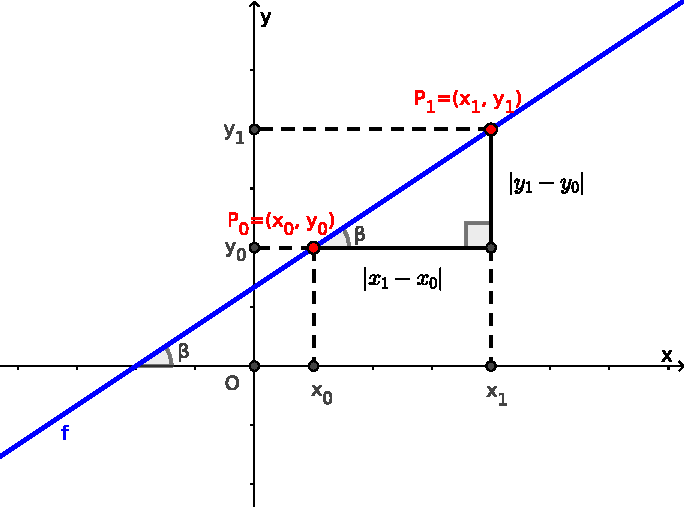
\includegraphics[width=8cm]{../Topicos/Figuras/coefangular.pdf}}
    \caption{Coeficiente angular}
  \end{figure}
  
  o coeficiente angular da reta que passa por estes dois pontos é dado por:
  \[a= \frac{y_1 - y_0}{x_1 - x_0} \ \ \ \text{ ou } \ \ \ a= \frac{y_0 - y_1}{x_0 - x_1} \ .\]
  
  De fato, dados dois pontos $P_0=(x_0, y_0)$, $P_1=(x_1, y_1)$, com $x_0 \neq x_1$, podemos encontrar a função $f(x)= ax+b$, cujo gráfico passa por estes dois pontos lembrando que ambos devem satisfazer a equação da função assim obtemos:
  \[ \begin{cases}
   y_0= ax_0 + b \\
   y_1= ax_1 + b
  \end{cases} \]
  logo $y_0 - ax_0= b$, substituindo na segunda equação decorre que:
  \[y_1= ax_1 + y_0 - ax_0 \Rightarrow y_1 - y_0= a(x_1 - x_0) \Rightarrow a= \frac{y_1 - y_0}{x_1 - x_0} \ . \]
  
  Este sistema linear sempre pode ser usado para encontrar a regra da função linear que passa por dois pontos dados.

  
  \begin{exem}
  Vamos determinar o coeficiente angular da reta que passa pelos pontos:
   \begin{enumerate}[a)]
    \item $P_0=(0,2)$ e $P_1=(-2,0)$
    \[a= \frac{y_1 - y_0}{x_1 - x_0}= \frac{0 - 2}{-2 - 0}= \frac{-2}{-2}= 1\]
    \item $P_0=(1,2)$ e $P_1=(-1,-2)$
    \[a= \frac{y_1 - y_0}{x_1 - x_0}= \frac{-2 - 2}{-1 - 1}= \frac{-4}{-2}= 2\]
   \end{enumerate}

  \end{exem}
  
  Quando dados dois pontos $P_0=(x_0, y_0)$, $P_1=(x_1, y_1)$, com $x_0 = x_1$, temos uma reta vertical, cuja equação é $x= a$ para algum $a \in \R$, que não é o gráfico de uma função, por isso não iremos detalhar este caso.
  
  Dadas duas funções lineares $f(x)=a_1 x + b_1$ e $g(x)= a_2 x + b_2$, tais que $f(x) \neq g(x)$, a partir da análise de seus coeficientes angulares podemos conhecer a posição relativa de seus gráficos. Nesta situação temos que dois casos especiais:
  \begin{itemize}
  \item Se $a_1= a_2$ então os gráficos de $f$ e $g$ são retas \textbf{paralelas};
  \item Se $a_1 \cdot a_2= -1$ então os gráficos de $f$ e $g$ são retas \textbf{perpendiculares}.
  \end{itemize}
  
  \begin{exem}
  Considere as funções $g(x)= -2x+4$, $f(x)= -2x+2$, $h(x)= \frac{-1}{-2}x+ 1,5$, pela análise com coeficientes angulares temos que os gráficos de $g$ e $f$ são retas paralelas e os gráficos $g$ e $h$ são retas perpendiculares, como podemos ver nos seguintes gráficos:
     \begin{figure}[H]
   \fbox{\subfigure[Retas paralelas]{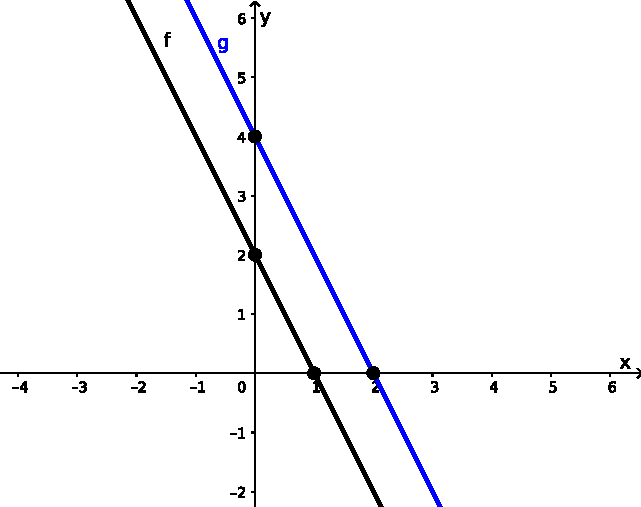
\includegraphics[width=7cm,height=6cm]{../Topicos/Figuras/retasparalelas.pdf}}}
   \fbox{\subfigure[Retas perpendiculares]{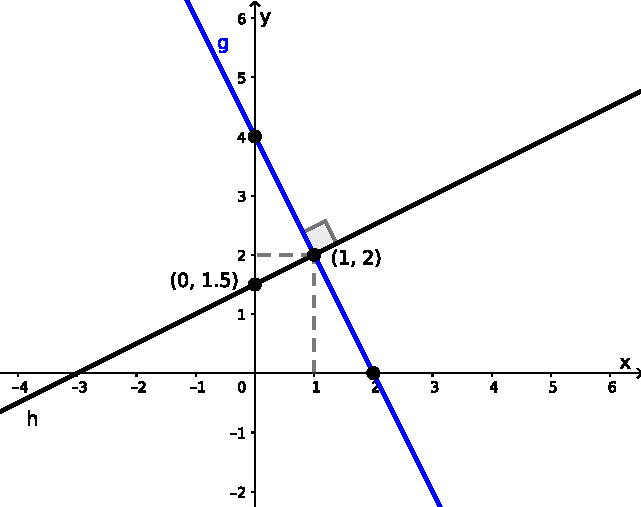
\includegraphics[width=7cm,height=6cm]{../Topicos/Figuras/retasperpendiculares.pdf}}}
  \end{figure} 
  \end{exem}

  
  
 \textbf{Zeros ou raízes das funções lineares}
 
 \vskip0.3cm
 \colorbox{azul}{
 \begin{minipage}{0.9\linewidth}
 \begin{center}
 Os zeros ou raízes de uma função $y= f(x)$ são os $x \in Dom(f)$ tais que $f(x)= 0$.
 \end{center}
 \end{minipage}}
 \vskip0.3cm
 
 Desta definição de \textbf{zeros} decorre que os zeros de uma função de 1º grau são as raízes da equação $ax+b=0$. Como esta equação é do 1º grau, ela possui uma única raiz, logo a função de 1º grau também possui uma única raiz, que denotaremos por $\tilde{x}$. Note que o ponto $(\tilde{x}, 0) \in \R^2$ é o ponto de interseção do gráfico da $f$ com o eixo $x$, assim podemos interpretar graficamente as raízes da nossa função como sendo os pontos de interseção do gráfico da função com o eixo das abscissas.

 \item Funções do 2º grau ou função quadrática

 São funções $f: \R \rightarrow \R$ dadas por:
 \[f(x)= ax^2 + bx + c\]

 Os \textbf{zeros} ou \textbf{raízes} das funções de 2º grau $f$, quando existem, são os $x \in dom(f)$ tais que $ax^2+bx+c=0$. Por ser esta uma equação do 2º grau temos três situações a considerar, dependendo do valor de $\Delta$:
 \[\destaque{\Delta= b^2 - 4*a*c}\]
 Se $\destaque{\Delta < 0}$ a função $f$ não possui raízes reais;

 Se $\destaque{\Delta = 0}$ a função $f$ possui uma única raiz real;

 Se $\destaque{\Delta > 0}$ a função $f$ possui duas raízes reais distintas, que podem ser calculadas resolvendo a equação de 2º grau através da fórmula para equações de 2º grau.
 
 Por definição, os zeros da função $f(x)= ax^2+bx+c$, são as raízes da equação $ax^2+bx+c=0$, já que estes são os valores de $x$ para os quais $f(x)=0$. Graficamente, quando estas funções possuem zeros eles são exatamente os pontos de interseção do gráfico da $f$ com o eixo $x$.

 Com relação a concavidade, o gráfico da função de 2º grau tem concavidade voltada \textbf{para cima} quando $\destaque{a > 0}$, e concavidade voltada \textbf{para baixo} quando $\destaque{a < 0}$.

 Em ambos os casos a função do 2º grau possui um vértice dado pela seguinte equação:

 \[ \destaque{V= \left(\frac{- b}{2a}, \frac{- \Delta}{4a} \right)} .\]

 No caso em que $a > 0$, o vértice do gráfico da função de 2º grau é um ponto de mínimo da função.

 No caso em que $a < 0$, o vértice do gráfico da função de 2º grau é um ponto de máximo da função.


  \begin{figure}[H]
   \fbox{\subfigure[$a > 0$ e $\Delta < 0$]{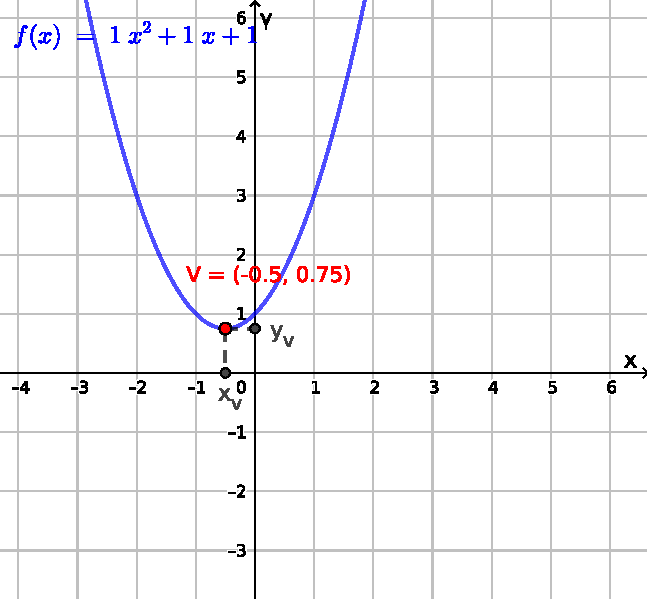
\includegraphics[width=7cm,height=6cm]{../Topicos/Figuras/f1.pdf}}}
   \fbox{\subfigure[$a > 0$ e $\Delta = 0$]{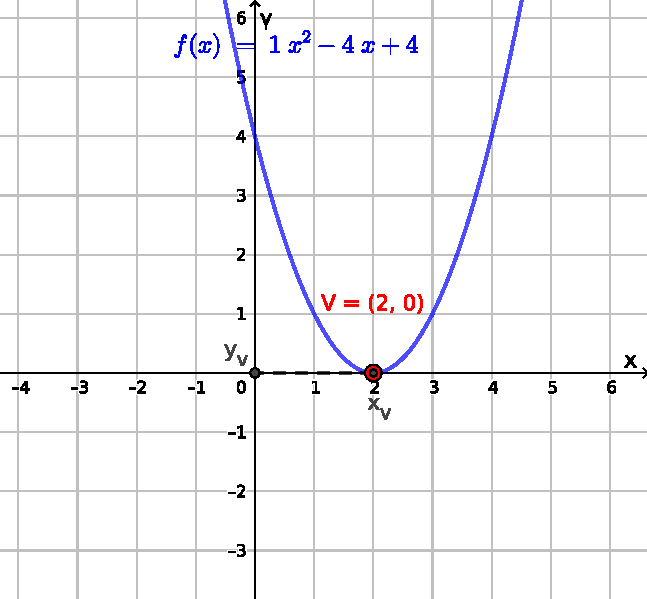
\includegraphics[width=7cm,height=6cm]{../Topicos/Figuras/f2.pdf}}}
  \end{figure} 
  
  \begin{figure}[H] 
   \fbox{\subfigure[$a > 0$ e $\Delta > 0$]{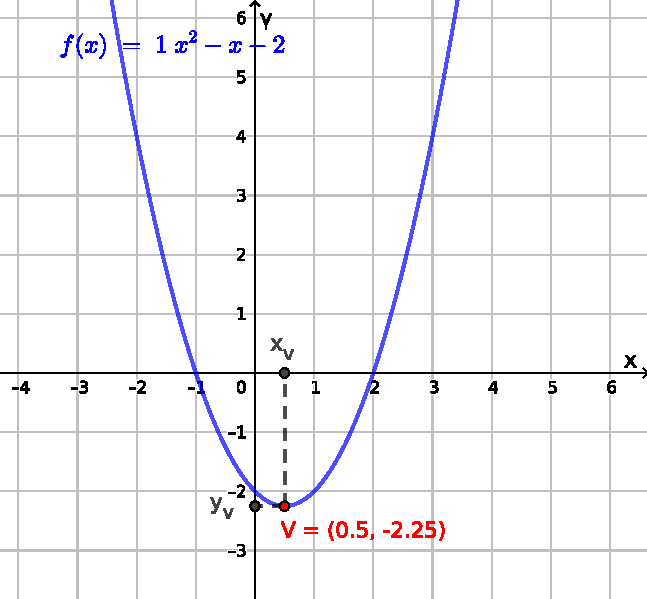
\includegraphics[width=7cm,height=6cm]{../Topicos/Figuras/f3.pdf}}}
   \fbox{\subfigure[$a < 0$ e $\Delta < 0$]{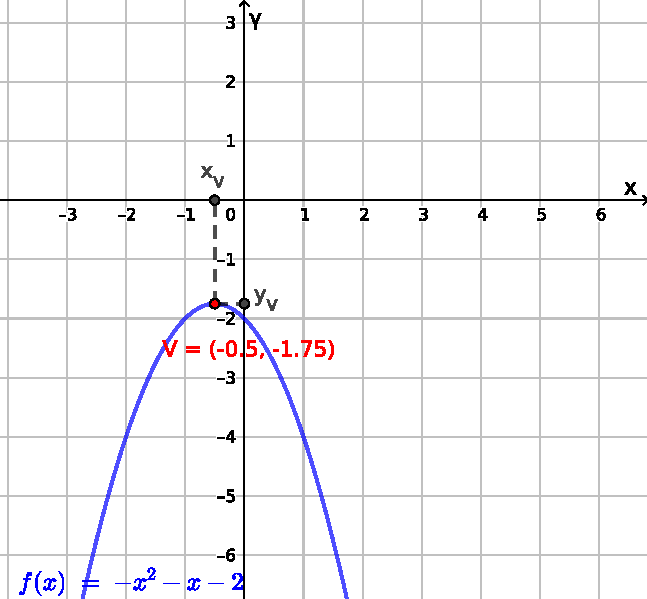
\includegraphics[width=7cm,height=6cm]{../Topicos/Figuras/f4.pdf}}}
  \end{figure}
  
   \begin{figure}[H]
   \fbox{\subfigure[$a < 0$ e $\Delta = 0$]{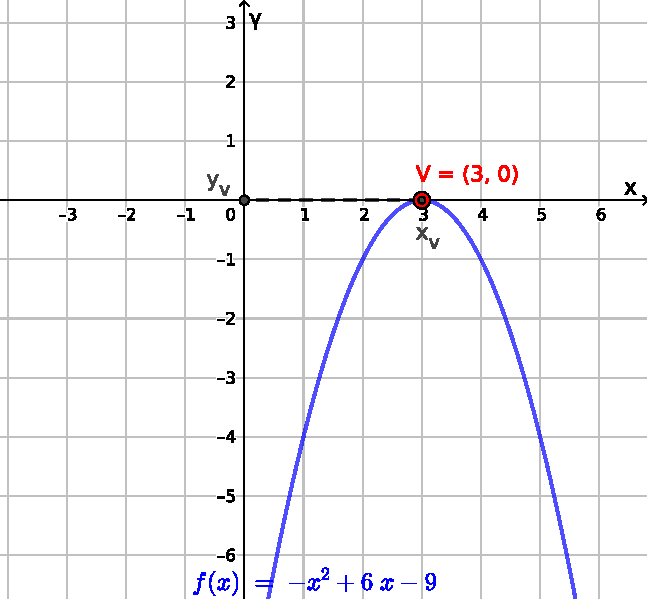
\includegraphics[width=7cm,height=6cm]{../Topicos/Figuras/f5.pdf}}}
   \fbox{\subfigure[$a < 0$ e $\Delta > 0$]{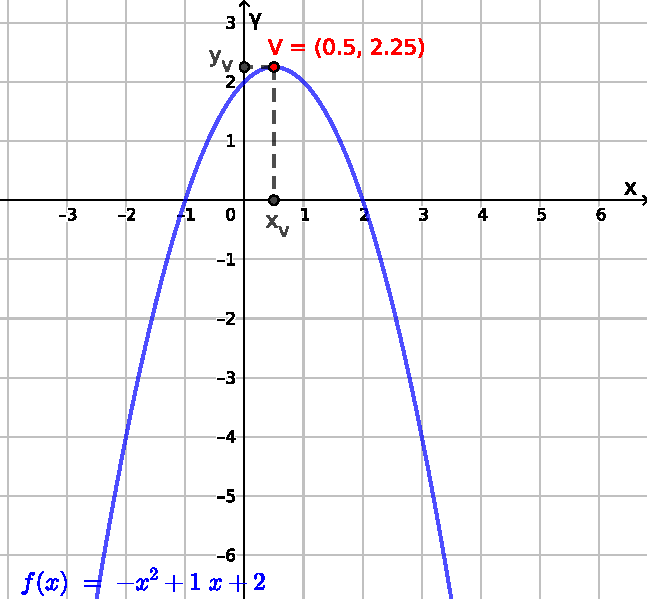
\includegraphics[width=7cm,height=6cm]{../Topicos/Figuras/f6.pdf}}}
   \caption{Gráficos de funções do 2º grau}
 \end{figure}


 \newpage
 \item Funções do 3º grau ou funções cúbicas

 São funções $f: \R \rightarrow \R$ dadas por:
 \[f(x)= ax^3 + bx^2 + cx + d .\]
 
 As \textbf{raízes} ou \textbf{zeros} das funções de 3º grau são os $x \in \R$ tais que $ax^3 + bx^2 + cx + d=0$. Assim as funções de 3º grau podem classificadas de acordo com suas raízes em 4 casos:
 \begin{enumerate}[(I)]
  \item 3 raízes reais distintas;
  \item 1 raiz real e duas raízes complexas;
  \item 3 raízes reais sendo duas delas iguais;
  \item 3 raízes reais iguais.
 \end{enumerate}
 Estes casos estão representados nos gráficos abaixo, onde consideramos sempre $a< 0$, o caso $a> 0$ é análogo.


   \begin{figure}[H]
   \fbox{\subfigure[$a < 0$]{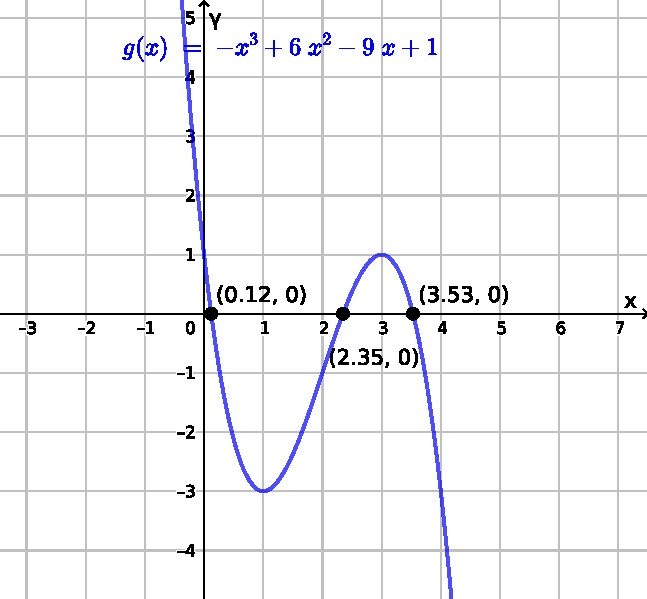
\includegraphics[width=7cm,height=5cm]{../Topicos/Figuras/g1.pdf}}}
   \fbox{\subfigure[$a < 0$]{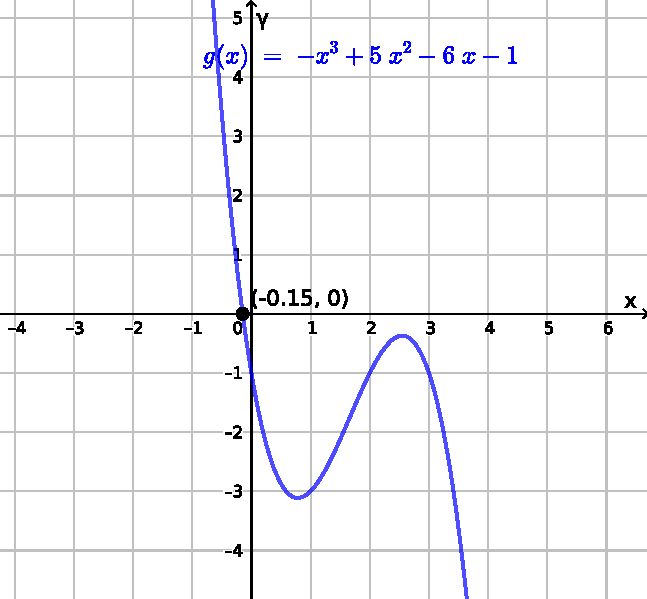
\includegraphics[width=7cm,height=5cm]{../Topicos/Figuras/g2.pdf}}}
   \end{figure}
   
  \begin{figure}[H]
   \fbox{\subfigure[$a < 0$]{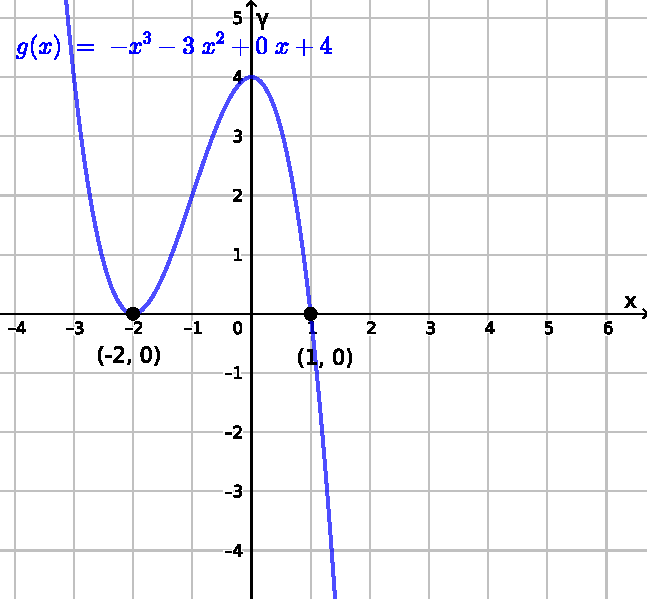
\includegraphics[width=7cm,height=5cm]{../Topicos/Figuras/g3.pdf}}}
   \fbox{\subfigure[$a < 0$]{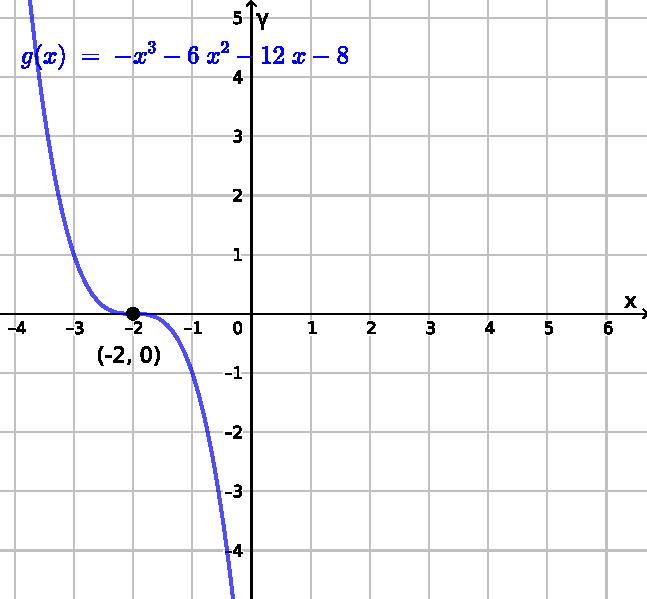
\includegraphics[width=7cm,height=5cm]{../Topicos/Figuras/g4.pdf}}}
   \caption{Gráficos de funções do 3º grau}
  \end{figure}
 
 \end{itemize}
 

  \subsection{Função modular}
  
  Considere a função $f: \R \rightarrow \R$, dada por $f(x)= |x|$, pela definição de módulo temos que $f$ é uma função definida por partes, da seguinte forma:

  \[f(x)= |x| = \begin{cases}
                 x, \text{ se } x \geq 0 \\
                 -x, \text{ se } x < 0
                \end{cases} \ .\]
 
 Cujo gráfico é dado por:
                
  \begin{figure}[H]
 \centering
    \fbox{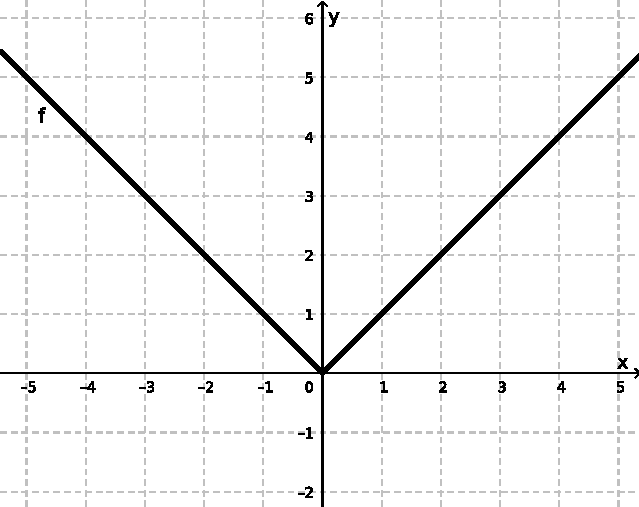
\includegraphics[width=8cm]{../Topicos/Figuras/funcaomodulo.pdf}}
    \caption{Gráfico da função módulo}
  \end{figure}
  
  Note que $f$ é decrescente no intervalo $]-\infty, 0[$, e crescente no intervalo $]0, \infty[$, e admite um mínimo em $x=0$.
  
  Consideramos agora a função $f_1: \R \rightarrow \R$ dada por $f_1(x)= |x+1|$, observe que:
  \[x+1 \geq 0 \Leftrightarrow  x \geq -1\]
  com isso podemos reescrever a função $f_1$ sem os módulos da seguinte forma:
  
  \[f_1(x)= \begin{cases}
                 x + 1, \text{ se } x \geq -1 \\
                 -x - 1, \text{ se } x < -1
                \end{cases} \ .\]
  Com isso a função modular pode ser vista como uma função linear por partes.
  
  Analogamente, para a função $f_2: \R \rightarrow \R$ dada por $f_2(x)= |x+1|+2$, temos que:
  \[x+1 \geq 0 \Leftrightarrow  x \geq -1\]
  com isso podemos reescrever a função $f_2$ sem os módulos da seguinte forma:
  
  \[f_2(x)= \begin{cases}
                 x + 3, \text{ se } x \geq -1 \\
                 -x + 1, \text{ se } x < -1
                \end{cases} \ .\]
  Com isso a função modular também pode ser vista como uma função linear por partes.
  
  Os gráficos das funções $f$, $f_1$ e $f_2$ estão dados na figura a seguir.  
  
  \begin{figure}[H]
 \centering
    \fbox{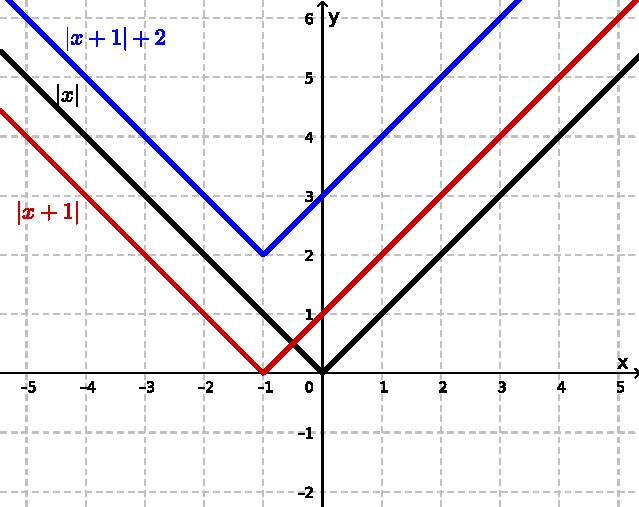
\includegraphics[width=8cm]{../Topicos/Figuras/funcaomodulo2.pdf}}
    \caption{Gráfico da função módulo}
  \end{figure}
  
  Comparando os gráficos das funções $f$ e $f_1$ notamos que ao somar uma constante "dentro" do módulo transladamos o gráfico da função $f$ no eixo $x$, e ao comparar as funções $f_1$ e $f_2$ percebemos que ao somar uma constante "fora" do módulo fazemos uma translação do gráfico da função $f_1$ em relação ao eixo $y$.
  
  \subsection{Mais algumas funções interessantes}
  
  \textbf{Função raíz quadrada}
  
  É a função $f: \R_{+} \to \R_{+}$ dada por $f(x)= \sqrt{x}$, cujo gráfico é:
  
   \begin{figure}[H]
 \centering
    \fbox{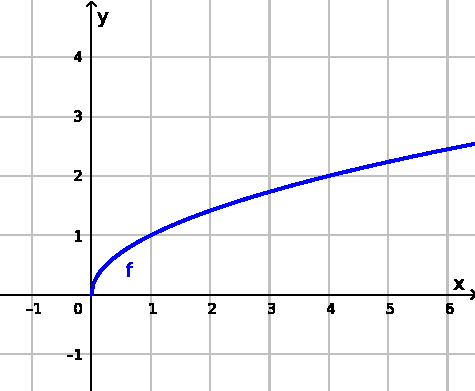
\includegraphics[width=6cm]{../Topicos/Figuras/funcaoraizquadrada.pdf}}
    \caption{Função raíz quadrada}
  \end{figure}
  
  Note que neste caso o domínio da função são apenas os números reais positivos, já que não existe raíz quadrada de número negativo.
  
  \newpage
  \textbf{Função raíz cúbica}
  
  É a função $f: \R \to \R$ dada por $f(x)= \sqrt[3]{x}$, cujo gráfico é:
  
   \begin{figure}[H]
 \centering
    \fbox{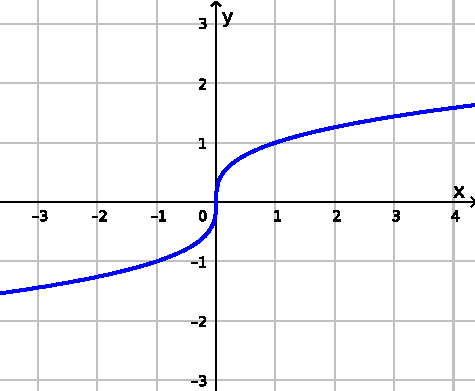
\includegraphics[width=6cm]{../Topicos/Figuras/funcaoraizcubica.pdf}}
    \caption{Função raíz cúbica}
  \end{figure} 
  
  \textbf{Função recíproca}
  
  É a função $f: \R \setminus \{0\} \to \R$ dada por $f(x)= \frac{1}{x}$, cujo gráfico é:
  
   \begin{figure}[H]
 \centering
    \fbox{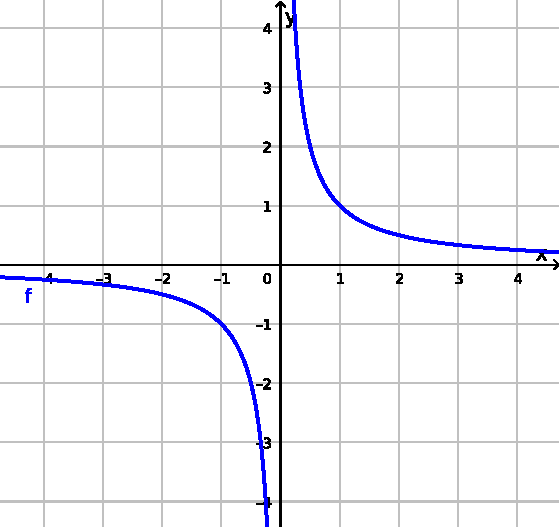
\includegraphics[width=6cm]{../Topicos/Figuras/funcaoreciproca.pdf}}
    \caption{Função recíproca}
  \end{figure}
  
  Neste caso o domínio da função é o conjunto $\R \setminus \{0\}$, pois não existe divisão por $0$ (zero).
  
  \newpage

  \textbf{Função floor}
  
  É a função $f: \R \to \R$ dada por $f(x)= \lfloor {x} \rfloor$, cujo gráfico é:
  
   \begin{figure}[H]
 \centering
    \fbox{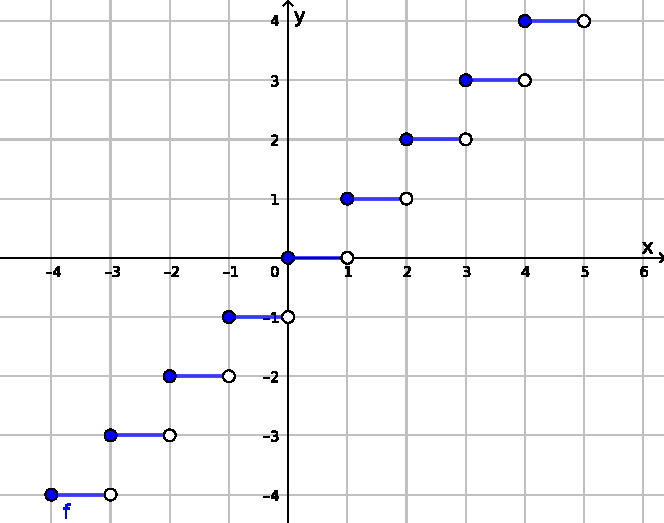
\includegraphics[width=6cm]{../Topicos/Figuras/funcaofloor.pdf}}
    \caption{Função floor}
  \end{figure}
  
  Esta função aplicada em um número $x$ tem como imagem a parte inteira do número $x$.
  
  \textbf{Função ceil}
  
  É a função $f: \R \to \R$ dada por $f(x)= \lceil {x} \rceil$, cujo gráfico é:
  
   \begin{figure}[H]
 \centering
    \fbox{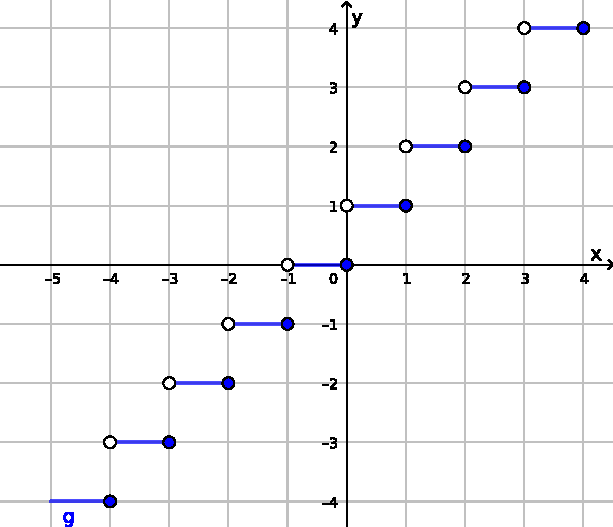
\includegraphics[width=6cm]{../Topicos/Figuras/funcaoceil.pdf}}
    \caption{Função ceil}
  \end{figure}
  
  Esta função aplicada em um número $x$ tem como imagem o menor inteiro maior ou igual a $x$.
  
  \section{Algumas propriedades das funções}
  
   \vskip0.3cm
 \colorbox{azul}{
 \begin{minipage}{0.9\linewidth}
 \begin{center}
  Dados $A, B \subset \R$ e uma função $f: A \rightarrow B$. 
  
  Dizemos que $f$ é uma \textbf{função crescente} em um intervalo $I \subset A$ se, para todo $x, y \in I$,
  \[ x < y \Rightarrow f(x) < f(y) \ .\]
  Dizemos que $f$ é uma \textbf{função descrescente} em um intervalo $I \subset A$ se, para todo $x, y \in I$,
  \[x < y \Rightarrow f(x) > f(y) \ .\]
  Dizemos que $f$ é uma \textbf{função constante} em um intervalo $I \subset A$ se, para todo $x, y \in I$,
  \[x \neq y \Rightarrow f(x) = f(y) \ .\]
 \end{center}
 \end{minipage}}
 \vskip0.3cm
 
 \begin{exem}
 Seja $f: \R \to \R$ uma função dada por $f(x)= ax + b$.
 
 Quando $\destaque{a > 0}$, dados $x_1 < x_2 \in dom(f)$, temos que:
 \[x_1 < x_2 \Rightarrow ax_1 < ax_2 \Rightarrow ax_1 + b < ax_2 + b \ ,\]
  portanto $f(x_1) < f(x_2)$, neste caso dizemos que $f$ é \textbf{crescente}. 

 Quando $\destaque{a < 0}$, dados $x_1 < x_2 \in dom(f)$, temos que:
 \[x_1 < x_2 \Rightarrow ax_1 > ax_2 \Rightarrow ax_1 + b > ax_2 + b \ ,\]
 portanto $f(x_1) > f(x_2)$, neste caso dizemos que $f$ é \textbf{decrescente}.
 
 Observe que no caso das funções de 1º grau a propriedade de ser crescente ou decrescente é válida em todo o domínio da função, nestes casos dizemos que é uma propriedade global da função.
 \end{exem}
 
 \begin{exem}
 Vamos retomar alguns dos nossos exemplos de funções para classificar como crescente, descrescente e constante. Para isso considere $x_1= -2$ e $x_2= 1$, neste caso, $x_1 < x_2$. 
  \begin{enumerate}[a)]
   \item Sendo $f(x)= \frac{1}{2}x + 1,5$, temos que 
   \[f(x_1)= f(-2)= \frac{1}{2}\cdot (-2) + 1,5= -1 + 1,5= 0,5\]
   \[f(x_2)= f(1)= \frac{1}{2} \cdot 1+\frac{3}{2}= \frac{4}{2}= 2\]
   logo $f(x_1)= 0,5 < 2= f(x_2)$. Portanto $f$ é crescente.
   \item Sendo $f(x)= -2x + 2$, temos que
   \[f(x_1)= f(-2)= -2 \cdot (-2) + 2= 4 + 2= 6\]
   \[f(x_2)= f(1)= -2 \cdot 1 + 2= 0\]
   logo $f(x_1)= 6 > 0 = f(x_2)$. Portanto $f$ é decrescente.
   \item Sendo $f(x)= 2$, temos que 
   \[f(x_1)= f(-2)= 2\]
   \[f(x_2)= f(1)= 2\]
   logo $f(x_1)= 2 = 2= f(x_2)$. Portanto $f$ é constante.
  \end{enumerate}
  Como já mostramos acima que para as funções lineares esta propriedade é global, para fazer esta classificação é suficiente testar dois valores de $x$ como fizemos acima.

 \end{exem}
 
 \begin{exem}
  Considere a função $f(x)= |x|$. Lembramos que esta função é definida por partes, por isso faremos a análise de crescimento e decrescimento em cada uma destas partes.
  
  Caso 1: Se $x < 0$, temos que $f(x)= -x$, logo se $x_1 < x_2$,
  \[x_1 < x_2 \Rightarrow -x_1 > -x_2 \Rightarrow f(x_1) > f(x_2) \ ,\]
  por exemplo, sendo $x_1= -3$ e $x_2= -2$ temos que $x_1 < x_2$,
  \[f(x_1)= f(-3)= -(-3)= 3 > 2= -(-2)= f(-2)= f(x_2) \ .\]
  
  Portanto se $x < 0$ temos que $f$ é decrescente.
  
  Caso 2: Se $x \geq 0$, temos que $f(x)= x$, logo se $x_1 < x_2$
  \[x_1 < x_2 \Rightarrow  f(x_1) < f(x_2) \ ,\]
  por exemplo, sendo $x_1= 2$ e $x_2= 3$ temos que $x_1 < x_2$,
  \[f(x_1)= 2 > 3= f(x_2) \ .\]
  
  Portanto se $x \geq 0$ temos que $f$ é crescente.
 \end{exem}


 
 \vskip0.3cm
 \colorbox{azul}{
 \begin{minipage}{0.9\linewidth}
 \begin{center}
  Dada um função $f: \R \rightarrow \R$. 
  
  Dizemos que $f$ é uma \textbf{função par} se, para todo $x \in R$,
  \[f(-x)= f(x) \ .\]
  Dizemos que $f$ é uma \textbf{função ímpar} se, para todo $x \in R$,
  \[f(-x)= - f(x) \ .\]
 \end{center}
 \end{minipage}}
 \vskip0.3cm

 
 \begin{exem}
  \begin{enumerate}[a)]
   \item A função $f(x)= x$ é uma função ímpar;
   \[f(-x)= -x= -f(x) \]
   \item A função $f(x)= x^2$ é uma função par;
   \[f(-x)= (-x)^2= x^2 = f(x) \]
   \item A função $f(x)= x^3$ é uma função ímpar.
   \[f(-x)= (-x)^3= -x^3= -f(x)\]
  \end{enumerate}
 \end{exem}
 
 \begin{exem}
  Vamos analisar a paridade de função modular $f(x)= |x|$.
  
  Caso 1: Se $x < 0$,
  \[f(x)= |x|= -x= f(-(x))= f(-x)\]
  por exemplo, $x= -2$, neste caso,
  \[f(x)= f(-2)= |-2|= -(-2)= 2= f(2)= f(-(-2))= f(-x) \ ;\]
  
  Caso 2: Se $x \geq 0$,
  \[f(x)= |x|= x= -(-x)= |-x|= f(-x)\]
  por exemplo, $x= 2$, neste caso,
  \[f(x)= f(2)= |2|= 2= -(-2)= |-2|= f(-2)= f(-x) \ .\]
  
  Portanto $f$ é uma função par.
 \end{exem}
  
  
  \subsection{Função inversa}

 Considere uma função $f: A \rightarrow B$, para $A, B \subset \R$. Se existir uma função $g: B \rightarrow A$ tal que:
 \[(g \circ f)(x)= x, \forall x \in A \ \ \ \text {e} \ \ \
 (f \circ g)(x)= x, \forall x \in B\]
 dizemos que $f$ é inversível e que $g$ é a inversa de $f$. Denotamos por $g= f^{-1}$.
 
 Ficamos com a seguinte pergunta: Quando existe $f^{-1}$? E a resposta é:
 
 \vskip0.3cm
 
 \colorbox{azul}{
 \begin{minipage}{0.9\linewidth}
 \begin{center}
 Uma função $f: A \to B$ é inversível se, e somente se, $f$ for bijetora, ou seja, injetora e sobrejetora.
 \end{center}
 \end{minipage}}

 \vskip0.3cm

\begin{exem}
 A função $f: \R \rightarrow \R$ dada por $f(x)= x+2$ é injetora, e sobrejetora portanto, existe uma função $g: \R \rightarrow \R$ dada por $g(x)= x-2$, tal que:
 \[h(x)= (f \circ g)(x)= f(g(x))= (x-2) + 2= x-2+2= x \Rightarrow (f \circ g)(x)= Id(x)\]
 \[\text{e}\]
 \[(g \circ f)(x)= g(f(x))= (x+2) - 2= x+2-2= x \Rightarrow (g \circ f)(x)= Id(x) ,\]
 logo $g= f^{-1}$ é a função inversa de $f$.

 \begin{figure}[H]
 \centering
    \fbox{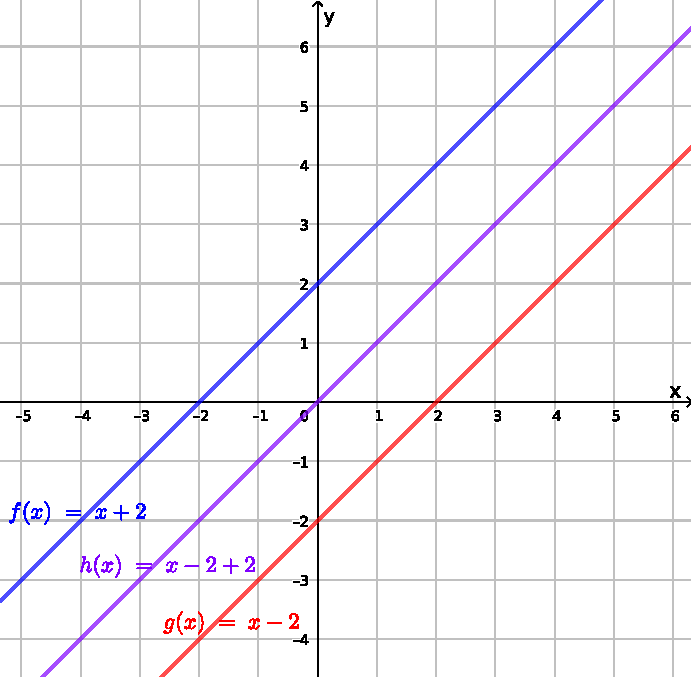
\includegraphics[width=8cm]{../Topicos/Figuras/funcao_composta.pdf}}
    \caption{Composta das funções $f$ e $g$}
  \end{figure}

\end{exem}

\newpage
 \section{Mudando os gráficos das funções}
 
 \subsection{Translação do gráfico das funções}
 
 Dados $A, B \subset \R$ e uma função $f(x): A \to B$, definimos a função translação de $f$ no eixo $y$, pela função $g(x): A \to B$, dada por \destaque{$g(x)= f(x) + c$}, onde $c \in \R$ é uma constante.
 
 \begin{exem}
  Considere a função $f(x): \R \to \R$, dada por $f(x)= x^2$. Defina as seguintes funções $g: \R \to \R$ dada por $g(x)= f(x) + 2= x^2 + 2$, e $h: \R \to \R$ dada por $h(x)= f(x) - 2= x^2 - 2$, observe na seguinte figura como estas translações alteram o gráfico da função $f$, note a função $g$ carregou o gráfico da $f$ duas unidades "para cima" no eixo $y$, já a função $h$ carregou o gráfico da $f$ duas unidades "para baixo" no eixo $y$.
  
 \begin{figure}[H]
   \fbox{\subfigure[Gráficos das funções $f$ e $g$]{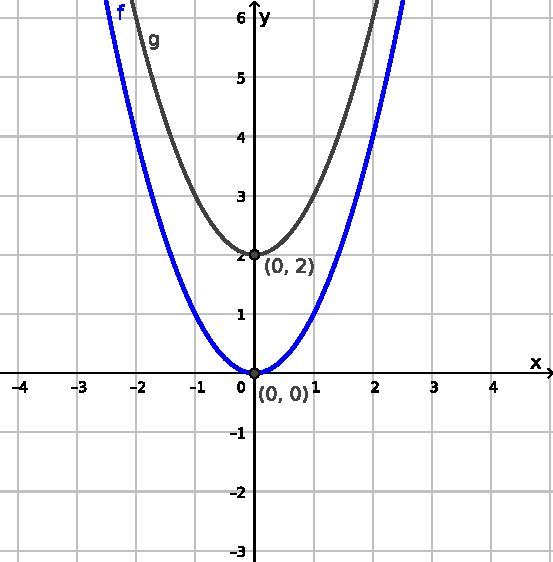
\includegraphics[width=7cm,height=6cm]{../Topicos/Figuras/translacaomais2.pdf}}}
   \fbox{\subfigure[Gráficos das funções $f$ e $h$]{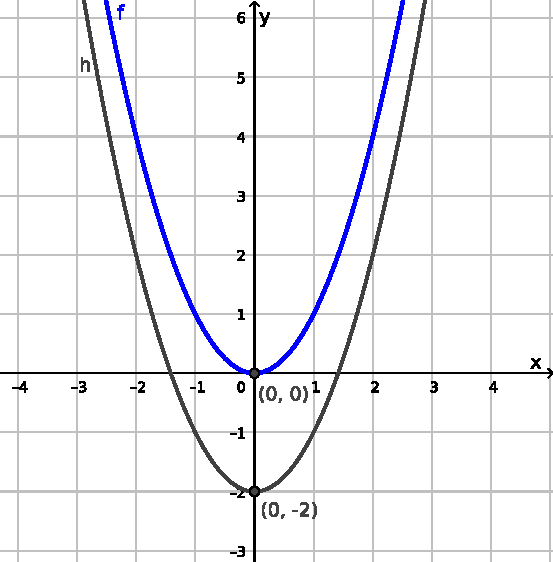
\includegraphics[width=7cm,height=6cm]{../Topicos/Figuras/translacaomenos2.pdf}}}
\caption{Translação no eixo $y$}
  \end{figure}
  
 \end{exem}

  Dados $A, B \subset \R$ e uma função $f(x): A \to B$, definimos a função translação de $f$ no eixo $x$, pela função $g(x): A \to B$, dada por \destaque{$g(x)= f(x + c)$}, onde $c \in \R$ é uma constante.
 
 \begin{exem}
  Considere a função $f(x): \R \to \R$, dada por $f(x)= x^2$. Defina as seguintes funções $g: \R \to \R$ dada por $g(x)= f(x + 2)= (x+2)^2$, e $h: \R \to \R$ dada por $h(x)= f(x-2)= (x-2)^2$, observe na seguinte figura como estas translações alteram o gráfico da função $f$, note a função $g$ carregou o gráfico da $f$ duas unidades "para à esquerda" no eixo $x$, já a função $h$ carregou o gráfico da $f$ duas unidades "para à direita" no eixo $x$.
  
 \begin{figure}[H]
   \fbox{\subfigure[Gráficos das funções $f$ e $g$]{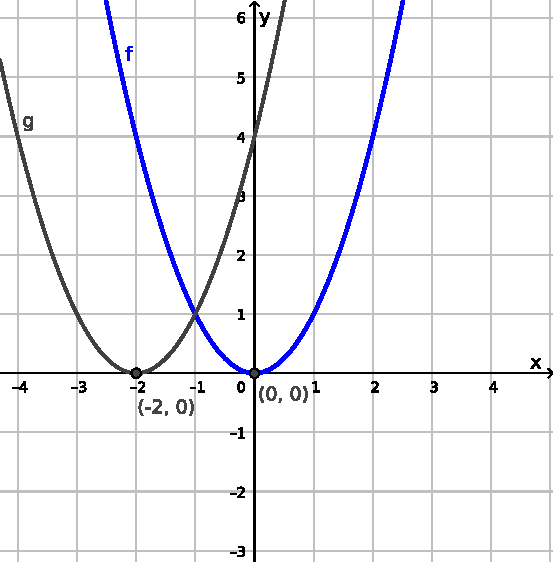
\includegraphics[width=7cm,height=6cm]{../Topicos/Figuras/translacaoXmais2.pdf}}}
   \fbox{\subfigure[Gráficos das funções $f$ e $h$]{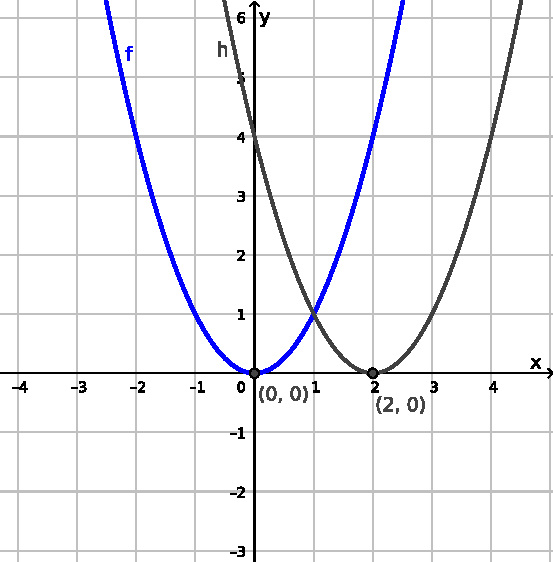
\includegraphics[width=7cm,height=6cm]{../Topicos/Figuras/translacaoXmenos2.pdf}}}
\caption{Translação no eixo $x$}
  \end{figure}
  
 \end{exem}
 
 \subsection{Reflexão do gráfico das funções}
 
 Dados $A, B \subset \R$ e uma função $f(x): A \to B$, definimos a função reflexão de $f$ no eixo $x$, pela função $g(x): A \to B$, dada por \destaque{$g(x)= -f(x)$}.
 
 \begin{exem}
  Considere a função $f(x): \R \to \R$, dada por $f(x)= x^2$. Defina a função $g: \R \to \R$ dada por $g(x)=-f(x)= -x^2$, note que $g$ é por definição a reflexão da função $f$ em torno do eixo $x$, como pode ser visto pela figura:
  
\begin{figure}[H]
   \centering
   \fbox{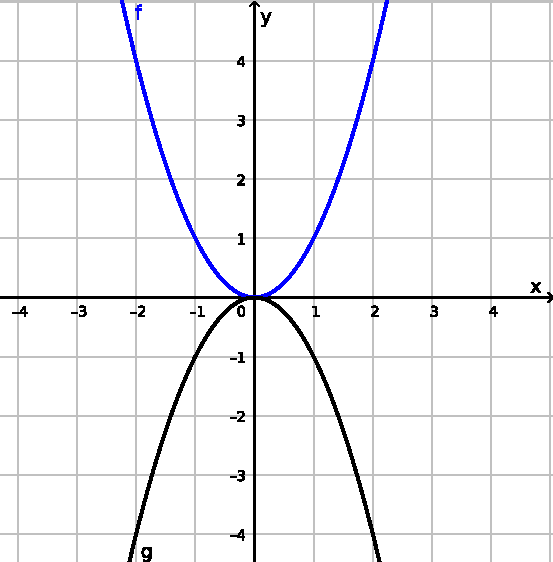
\includegraphics[width=7cm]{../Topicos/Figuras/reflexaoemX.pdf}}
   \caption{Reflexão no eixo $x$}
  \end{figure}
  
 \end{exem}

 
 Dados $A, B \subset \R$ e uma função $f(x): A \to B$, definimos a função reflexão de $f$ no eixo $y$, pela função $g(x): A \to B$, dada por \destaque{$g(x)= f(-x)$}.
 
 \begin{exem}
  Considere a função $f(x): \R \to \R$, dada por $f(x)= x^3$. Defina a função $g: \R \to \R$ dada por $g(x)=f(-x)= (-x)^3$, note que $g$ é por definição a reflexão da função $f$ em torno do eixo $y$, como pode ser visto pela figura:
  
\begin{figure}[H]
   \centering
   \fbox{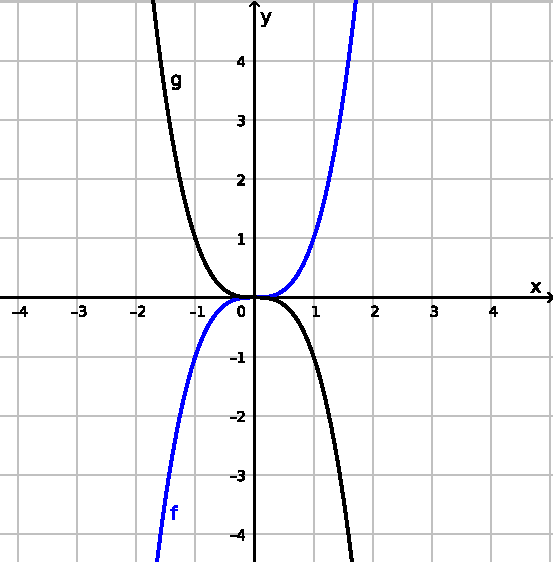
\includegraphics[width=7cm]{../Topicos/Figuras/reflexaoemY.pdf}}
   \caption{Reflexão no eixo $y$}
  \end{figure}
  
 \end{exem}
 
 Resumindo, dados $A, B \subset \R$, uma função $f(x): A \to B$, e uma constante $c \in \R$ obtemos as seguintes funções $g: A \to B$:
  \begin{table}[H]
 \centering
 \begin{tabular}{|c|c|} \hline
 \rowcolor{cinza}
  Mudança & Função \\\hline
  Translação no eixo $y$ & $g(x)= f(x)+ c$ \\\hline
  Translação no eixo $y$ & $g(x)= f(x)- c$ \\\hline
  Translação no eixo $x$ & $g(x)= f(x+ c)$ \\\hline
  Translação no eixo $x$ & $g(x)= f(x- c)$ \\\hline
  Reflexão no eixo $x$ & $g(x)= -f(x)$ \\\hline
  Reflexão no eixo $y$ & $g(x)= f(-x)$ \\\hline
 \end{tabular}
\end{table}
 
  \newpage
  \section{Trigonometria}

 \subsection{Triângulo retângulo}

  Considere o triângulo retângulo, (triângulo que possui um de seus ângulos internos medindo $90 \degree$), como na figura abaixo:
  \begin{figure}[H]
   \centering
   \fbox{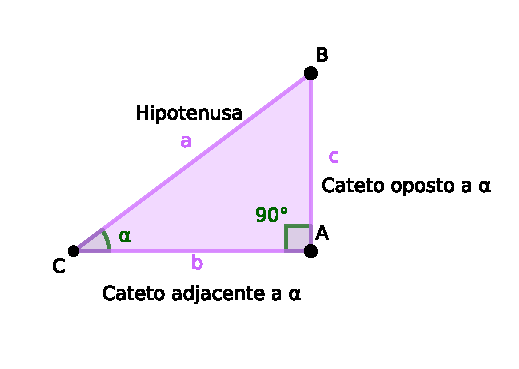
\includegraphics[width=7cm]{../Topicos/Figuras/triangulo_retangulo.pdf}}
   \caption{Triângulo retângulo}
  \end{figure}
 para este triângulo temos que é válido o seguinte teorema:

 \vskip0.3cm

\colorbox{azul}{
 \begin{minipage}{0.9\linewidth}
 \begin{center}
 \textbf{Teorema de Pitágoras}
  \[a^2= b^2 + c^2.\]
 \end{center}
 \end{minipage}}

 \vskip0.3cm

 Este é um resultado importante, já que com ele é possível encontrar o valor de um dos lados do triângulo, nos casos em que não temos todos os lados dados.

 Para este triângulo, as funções seno, cosseno e tangente são dadas pelas seguintes razões trigonométricas, nesta ordem:

 \vskip0.3cm

\colorbox{azul}{
 \begin{minipage}{0.9\linewidth}
 \begin{center}
 \textbf{Funções trigonométricas}
  \begin{eqnarray*}
   sen(\alpha)= \frac{c}{a}= \frac{CO}{HI} \ ; \ \ cos(\alpha)= \frac{b}{a}= \frac{CA}{HI} \ ; \ \ tan(\alpha)= \frac{c}{b}= \frac{CO}{CA}.
 \end{eqnarray*}
 \end{center}
 \end{minipage}}

 \vskip0.3cm

 Como a soma dos ângulos internos de um triângulo é $180 \degree$, e estamos aqui tratando de um triângulo retângulo, decorre que neste caso $0 \degree \leqslant \alpha \leqslant 90 \degree$. Porém estas funções estão definidas para qualquer número real, mas para um primeiro estudo é suficiente conhecer seus valores para os ângulos $0 \degree \leqslant \alpha \leqslant 360 \degree$.

 Destacamos aqui os valores do seno, cosseno e tangente dos \emph{ângulos notáveis} que são os mais utilizados:

 \begin{table}[H]
 \centering
 \begin{tabular}{|c|c|c|c|c|c|} \hline
 \rowcolor{cinza}
               & $0 \degree$  & $30 \degree$  & $45 \degree$  & $60 \degree$ & $90 \degree$  \\\hline
  \textbf{sen} & $0$ &$\frac{1}{2}$ & $\frac{\sqrt{2}}{2}$ & $\frac{\sqrt{3}}{2}$ & $1$ \\\hline
  \textbf{cos} & $1$ & $\frac{\sqrt{3}}{2}$ & $\frac{\sqrt{2}}{2}$ & $\frac{1}{2}$ & $0$ \\\hline
  \textbf{tan} & $0$ & $\frac{\sqrt{3}}{3}$ & $1$ & $\sqrt{3}$ & $\nexists$ \\\hline
 \end{tabular}
\end{table}
 Na próxima seção veremos como utilizar estes valores para calcular seno, cosseno e tangente de ângulos maiores que $90 \degree$.

\subsection{Círculo trigonométrico}

 No plano cartesiano, consideremos um círculo de centro na origem e raio $1$, neste círculo representamos as imagens das funções trigonométricas aplicadas à  $0 \degree \leqslant \alpha \leqslant 360 \degree$. Como mostra a seguinte figura:
 \begin{figure}[H]
   \centering
   \fbox{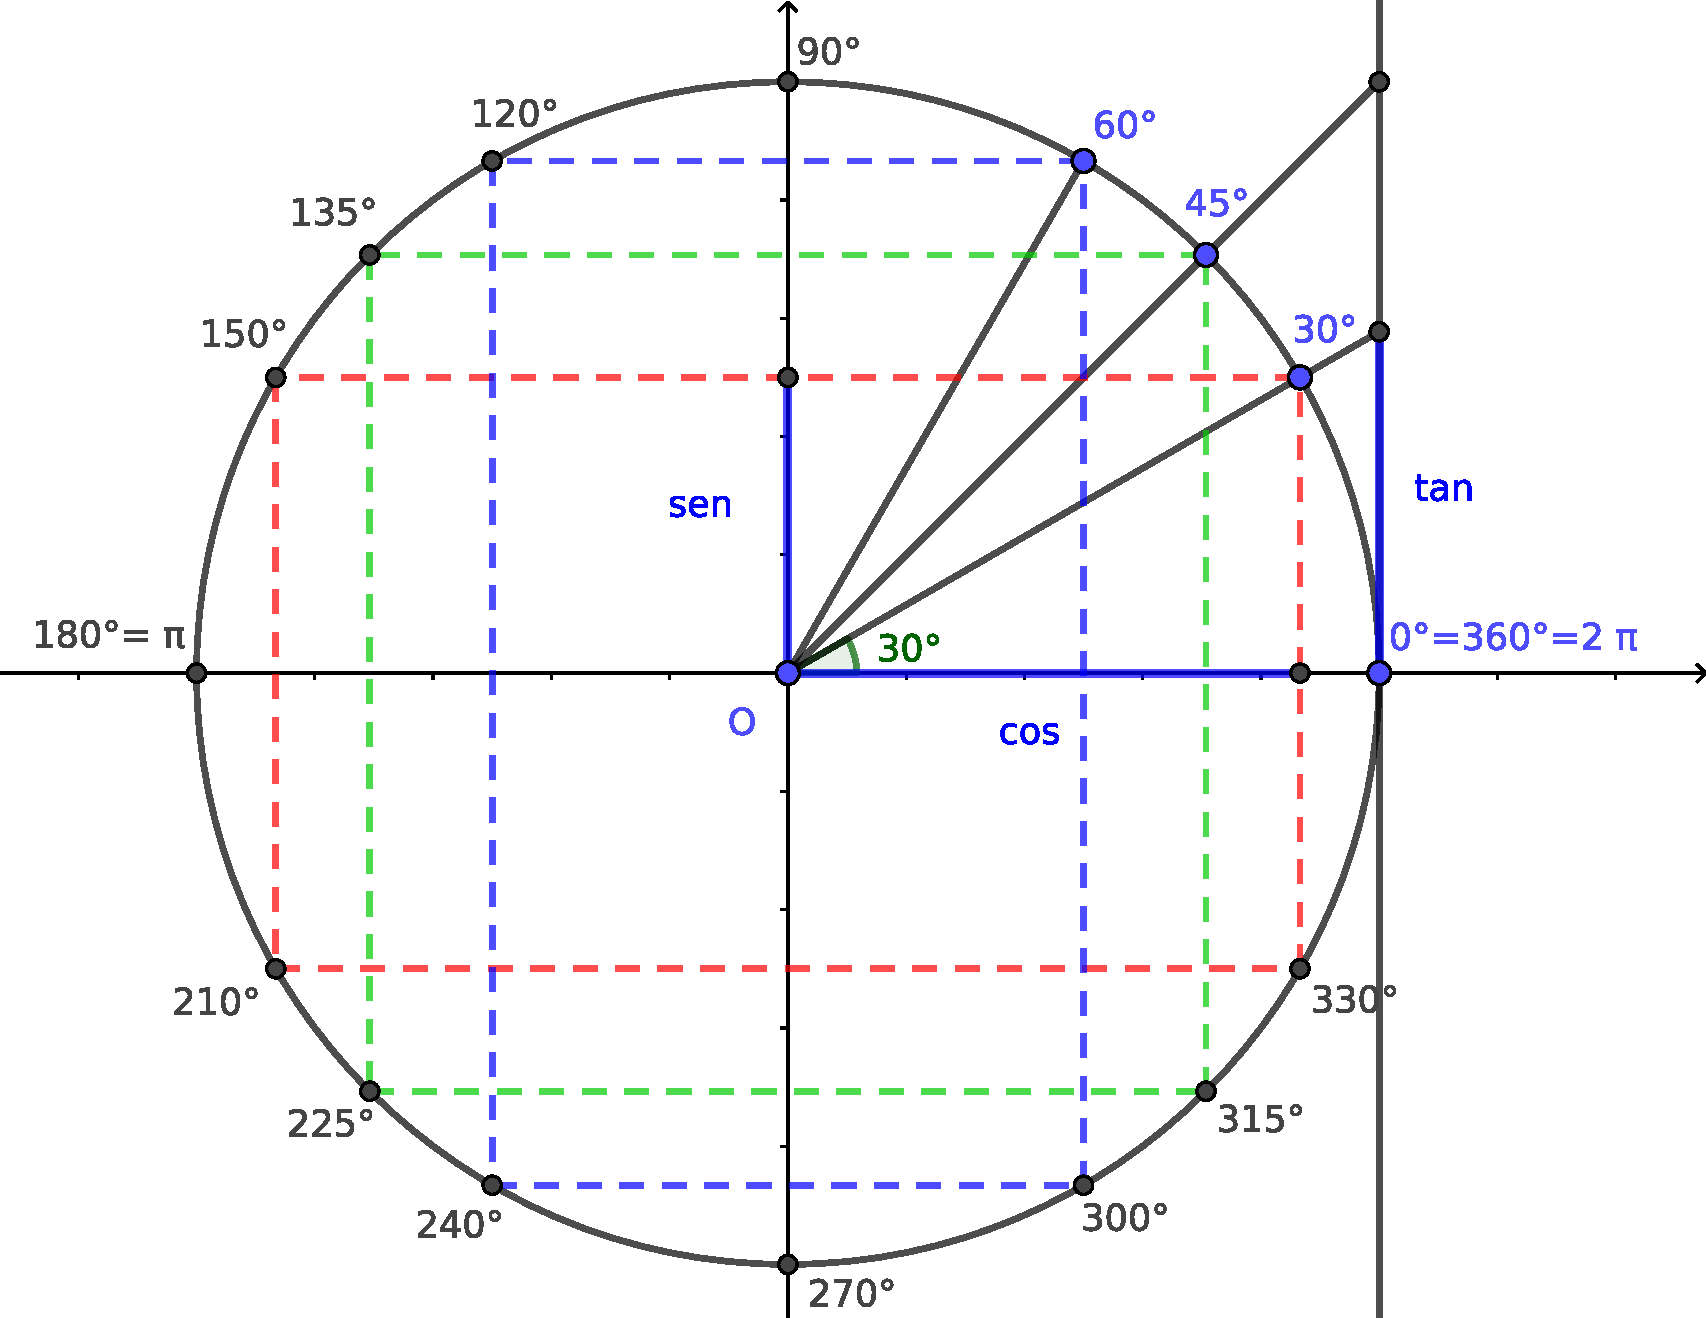
\includegraphics[width=9cm]{../Topicos/Figuras/circulo_trigonometrico.pdf}}
   \caption{Círculo trigonométrico}
  \end{figure}

  A partir do círculo trigonométrico concluímos que:

  \begin{table}[H]
 \centering
 \begin{tabular}{|c|c|c|c|} \hline
 \rowcolor{cinza}
               &  $120\degree$  & $135\degree$  &  $150\degree$ \\\hline
  \textbf{sen} & $sen(60\degree)$ &$sen(45\degree)$ & $sen(30\degree)$  \\\hline
  \textbf{cos} & $-cos(60\degree)$ &$-cos(45\degree)$ & $-cos(30\degree)$  \\\hline
  \textbf{tan} & $-tan(60\degree)$ &$-tan(45\degree)$ & $-tan(30\degree)$  \\\hline
 \end{tabular}
\end{table}

 \begin{table}[H]
 \centering
 \begin{tabular}{|c|c|c|c|} \hline
 \rowcolor{cinza}
                & $210\degree$ & $225\degree$  & $240\degree$  \\\hline
  \textbf{sen} &  $-sen(30\degree)$ & $-sen(45\degree)$ & $-sen(60\degree)$  \\\hline
  \textbf{cos} &  $-cos(30\degree)$ & $-cos(45\degree)$ & $-cos(60\degree)$  \\\hline
  \textbf{tan} &  $tan(30\degree)$ & $tan(45\degree)$ & $tan(60\degree)$   \\\hline
 \end{tabular}
\end{table}

 \begin{table}[h]
 \centering
 \begin{tabular}{|c|c|c|c|} \hline
 \rowcolor{cinza}
               & $300\degree$ & $315\degree$ & $330\degree$ \\\hline
  \textbf{sen} & $sen(60\degree)$ & $sen(45\degree)$ & $sen(30\degree)$ \\\hline
  \textbf{cos} & $cos(60\degree)$ & $cos(45\degree)$ & $cos(30\degree)$  \\\hline
  \textbf{tan} & $-tan(60\degree)$ & $-tan(45\degree)$ & $-tan(30\degree)$  \\\hline
 \end{tabular}
\end{table}


  Os ângulos podem também ser representados em radianos, respeitando a seguinte relação:

  \[\destaque{\pi \text{ radianos}= 180 \degree}\]

  Usando esta relação podemos transformar graus para radianos e radianos para graus, vamos ver dois exemplos:

  \begin{exem}
   Qual a medida em graus do ângulo que mede $\frac{\pi}{4} rad$?

   \underline{Resolução:}

   Sabemos que $\pi rad= 180\degree$, portanto usando a regra de 3 abaixo conseguimos encontrar o valor em graus deste ângulo:
   \begin{eqnarray*}
  \text{Graus} & & \text{Radianos} \\
   180 & = & \pi\\
  x & = & \frac{\pi}{4}
 \end{eqnarray*}
 usando a propriedade da proporcionalidade, ou seja, multiplicando cruzado temos:

 $180 \cdot \frac{\pi}{4}= \pi \cdot x \Rightarrow \pi \cdot x= \frac{180 \pi}{4} \Rightarrow x= \frac{45 \pi}{\pi} \Rightarrow x= 45\degree$.

 \fim
  \end{exem}

  \begin{exem}
   Qual a medida em radianos do ângulo que mede $30\degree$?

   \underline{Resolução:}

   Sabemos que $\pi rad= 180\degree$, portanto usando a regra de 3 abaixo conseguimos encontrar o valor em graus deste ângulo:
   \begin{eqnarray*}
  \text{Graus} & & \text{Radianos} \\
   180 & = & \pi\\
  30 & = & x
 \end{eqnarray*}
 usando a propriedade da proporcionalidade, ou seja, multiplicando cruzado temos:

 $180 \cdot x= \pi \cdot 30 \Rightarrow x= \frac{30 \pi}{180} \Rightarrow x= \frac{\pi}{6} rad$.

 \fim
  \end{exem}

 \newpage

 \subsection{Identidades trigonométricas}
 
 \textbf{Identidades de quociente}
 
 \[tan(x)= \dfrac{sen(x)}{cos(x)} \qquad cotan(x)= \dfrac{cos(x)}{sen(x)}\]
 
 \vskip0.5cm
 \textbf{Identidades recíprocas}
 
 \[sec(x)= \dfrac{1}{cos(x)} \qquad 
   csc(x)= \dfrac{1}{sen(x)} \qquad 
   cotan(x)= \dfrac{1}{tan(x)}\]
 
 \vskip0.5cm
 \textbf{Identidades pitagóricas}
 
 \[sen^2(x) + cos^2(x)= 1 \qquad 
   tan^2(x)+ 1= sec^2(x) \qquad 
   cotan^2(x)+1=cosec^2(x)\]
 
 \vskip0.5cm
 \textbf{Identidades associadas à paridade}
 
 \[sen(-x)= -sen(x) \qquad cos(-x)= cos(x) \qquad tan(-x)=-tan(x)\]
 
 \vskip0.5cm
 \textbf{Identidades de arcos complementares}
 
 \[sen \left(\frac{\pi}{2} - x \right)= cos(x) \qquad 
   cos \left(\frac{\pi}{2} - x \right)= sen(x)\]
 
 \[tan \left(\frac{\pi}{2} - x \right)= cotan(x) \qquad
   cotan \left(\frac{\pi}{2} - x \right)= tan(x)\]
 
 \[cosec \left(\frac{\pi}{2} - x \right)= sec(x) \qquad
   sec \left(\frac{\pi}{2} - x \right)= cosec(x)\]
 

\vskip0.5cm
 \textbf{Fórmulas de adição e subtração}
 
 Seno
 \begin{eqnarray*}
  sen(a+b)&=&sen(a)\cdot cos(b)+sen(b)\cdot cos(a) \\
  sen(a-b)&=&sen(a)\cdot cos(b)-sen(b)\cdot cos(a)
 \end{eqnarray*}
 
 Cosseno
 \begin{eqnarray*}
  cos(a+b)&=&cos(a)\cdot cos(b)-sen(a)\cdot sen(b) \\
  cos(a-b)&=&cos(a)\cdot cos(b)+sen(a)\cdot sen(b)
 \end{eqnarray*}
 
 Tangente
 \begin{eqnarray*}
  tan(a+b)&=& \frac{tan(a)+tan(b)}{1-tan(a)\cdot tan(b)} \\
  tan(a-b)&=& \frac{tan(a)-tan(b)}{1-tan(a)\cdot tan(b)}
 \end{eqnarray*}

  
  \section{Funções trigonométricas}

  As funções trigonométricas fazem parte do grupo de funções periódicas, que são as funções que satisfazem a seguinte definição.
  
  \begin{defi}
   Uma função $f: \R \rightarrow \R$ é denominada \textbf{periódica} quando existe um número real positivo $P$ tal que
   \[f(x + P)= f(x)\]
   para todo $x$ no domínio da $f$. O menor número real positivo $P$ que satisfaz esta propriedade é denominado período de $f$.
  \end{defi}

  Vamos definir as funções trigonométricas no maior subconjunto real possível, e estudar o comportamento de seus gráficos.

  \todo{ períodos, amplitude, intervalo de bijetividade, função inversa}

  \begin{itemize}
  \item Função Seno: $f: \R \rightarrow [-1, 1]$ dada por $f(x)= sen (x)$, cujo gráfico é:

  \begin{figure}[H]
  \centering
    \fbox{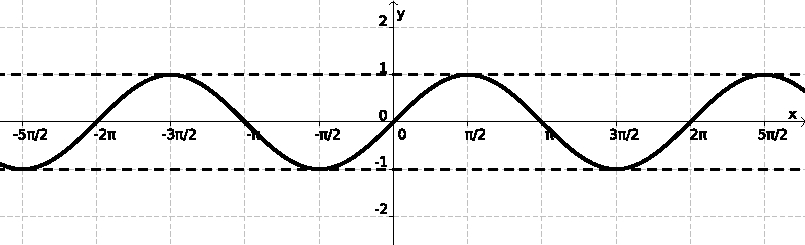
\includegraphics[width=10cm]{../Topicos/Figuras/sen.pdf}}
    \caption{Gráfico da função $f(x)= sen (x)$}
  \end{figure}

  \item Função Cosseno: $f: \R \rightarrow [-1, 1]$ dada por $f(x)= cos (x)$, cujo gráfico é:

  \begin{figure}[H]
  \centering
    \fbox{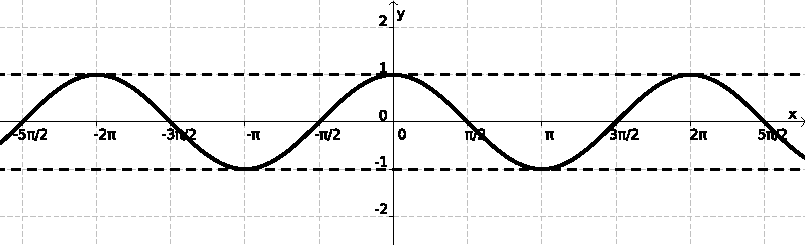
\includegraphics[width=10cm]{../Topicos/Figuras/cos.pdf}}
    \caption{Gráfico da função $f(x)= cos (x)$}
  \end{figure}
  
  Geométricamente podemos observar que o comportamento do gráfico das funções seno o cosseno no intervalo $[0, 2\pi]$ se repete em cada intervalo de comprimento $2\pi$. Isso pode ser visualizado também olhando para o círculo trigonométrico, por exemplo quando estamos olhando para um ângulo $\theta= 4\pi + \frac{\pi}{4}$ estamos apenas dando duas voltas no círculo trigonométrico e andando mais $\frac{\pi}{4}$, por isso:
  \[sen(4\pi + \frac{\pi}{4})= sen(\frac{\pi}{4}) \ ,\]
  \[cos(4\pi + \frac{\pi}{4})= cos(\frac{\pi}{4}) \ , \]
  funções com esta propriedade de repetição de comportamento são denominadas funções periódicas, e o intervalo que se repete é chamado de período.
  
  Por interpretação do círculo trigonométrico vemos que, para todo $x \in \R$:
  \[sen(x + 2 \pi)= sen(x) \ ,\]
  \[cos(x + 2\pi)= cos(x) \ , \]
  logo as funções seno e cosseno são de fato funções períodicas de período $2\pi$.
  
  \item Função Tangente: $f: \R \setminus \{\frac{k\pi}{2} | k \in \Z\} \rightarrow \R$ dada por $f(x)= tan (x)$, cujo gráfico é:

  \begin{figure}[H]
  \centering
    \fbox{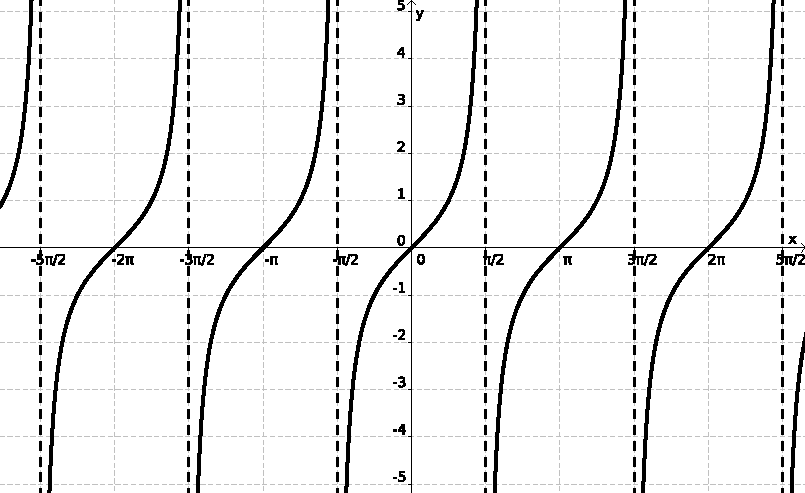
\includegraphics[width=10cm]{../Topicos/Figuras/tan.pdf}}
    \caption{Gráfico da função $f(x)= tan (x)$}
  \end{figure}
    
  Lembramos que $tan(x)= \frac{sen(x)}{cos(x)}$, logo podemos entender o domínio da função tangente como o conjunto dos $x \in \R$ tais que $cos(x) \neq 0$.
  
  Note que o comportamento do gráfico da função tangente no intervalo $]-\frac{\pi}{2}, \frac{\pi}{2}[$ se repete indefinadamente, e ainda
  \[tan(x)= tan(x + \pi)\]
  donde concluímos que a função tangente é uma função períodica de período $\pi$.

  \item Função Cossecante: $f: \R \setminus \{ k\pi | k \in \Z\} \rightarrow \R$ dada por $f(x)= csc(x)$, o gráfico desta função é: 

  \begin{figure}[H]
  \centering
    \fbox{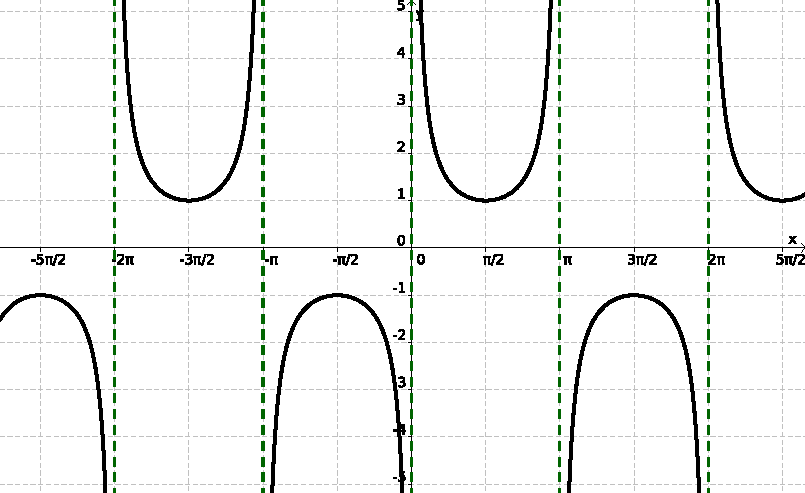
\includegraphics[width=10cm]{../Topicos/Figuras/csc.pdf}}
    \caption{Gráfico da função $f(x)= csc(x)$}
  \end{figure}
    
  Como $csc(x)= \dfrac{1}{sen (x)}$ o domínio da função cossecante é exatamente o conjunto dos $x \in \R$ tais que $sen(x) \neq 0$.
  
  Ao observar o gráfico da função cossecante notamos que o gráfico da função no intervalo $]0, \pi[ \cup ] \pi, 2 \pi[$ se repete indefinidamente, e ainda
  \[csc(x + 2\pi)= csc(x) \ , \]
  logo esta é uma função periódica, com período $2\pi$.

  \item Função Secante: $f: \R \setminus \{\frac{k\pi}{2} | k \in \Z\} \rightarrow \R$ dada por $f(x)= sec(x)$, com gráfico dado por:

  \begin{figure}[H]
  \centering
    \fbox{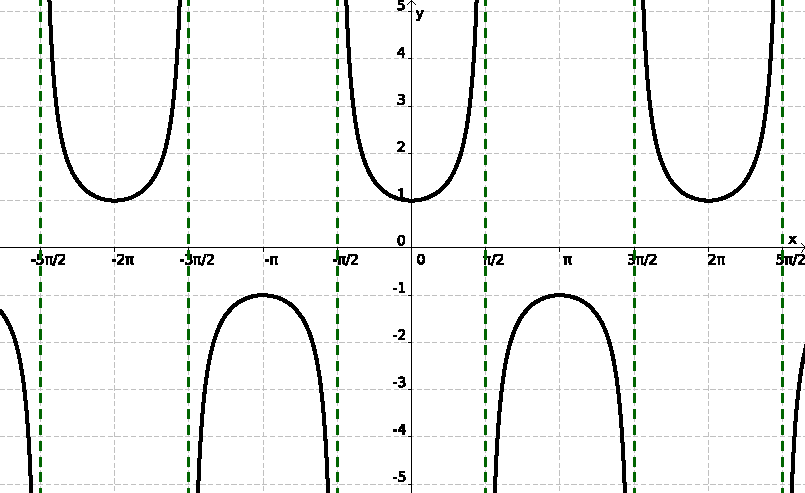
\includegraphics[width=10cm]{../Topicos/Figuras/sec.pdf}}
    \caption{Gráfico da função $f(x)= sec(x)$}
  \end{figure}
  
  Como $sec(x)= \dfrac{1}{cos (x)}$ o domínio da função secante é o conjunto dos $x \in \R$ tais que $cos(x) \neq 0$.
  
  Ao observar o gráfico da função secante notamos que o intervalo que se repete neste caso é $]\frac{-\pi}{2}, \frac{\pi}{2}[ \cup ] \frac{\pi}{2}, \frac{3\pi}{2}[$, e ainda que
  \[sec(x + 2\pi)= sec(x) \ ,\]
  logo esta é uma função periódica com período $2\pi$.

  \item Função Cotangente: $f: \R \setminus \{ k\pi | k \in \Z\} \rightarrow \R$ dada por $f(x)= cotan(x)$, cujo gráfico é:

  \begin{figure}[H]
  \centering
    \fbox{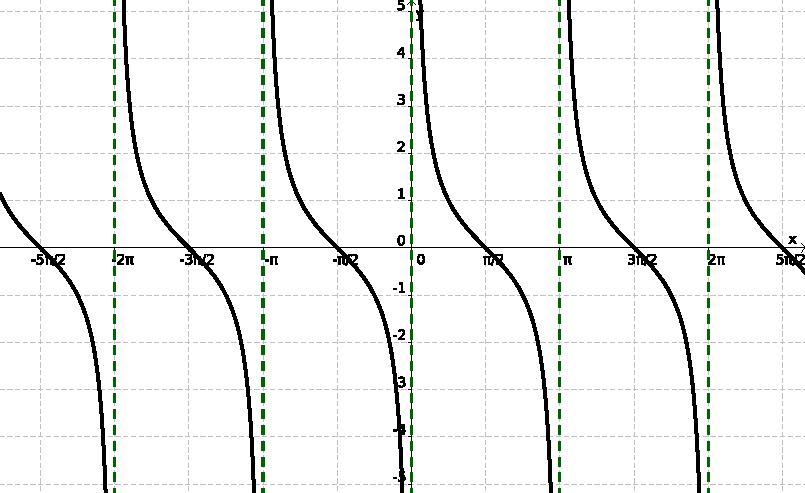
\includegraphics[width=10cm]{../Topicos/Figuras/cot.pdf}}
    \caption{Gráfico da função $f(x)= cotan(x)$}
  \end{figure}
  
  Lembramos que $cotan(x)= \dfrac{cos(x)}{sen(x)}$ logo o domínio da função cotangente é o conjunto dos $x \in \R$ tais que $sen(x) \neq 0$.
  
  Já no gráfico da função cotangente vemos a repetição do comportamento do intervalo $]0, \pi[$, e temos que
  \[cotan(x + \pi)= cotan(x)\]
  portanto esta é uma função periódica de período $\pi$.

  \textbf{Funções Inversas}
  
  As funções trigonométricas admitem inversas quando restringimos seus domínios a um único período da função, assim temos por exemplo as seguintes funções:
  
  \item Função Arco Seno: $f: [-1, 1] \rightarrow [\frac{-\pi}{2}, \frac{\pi}{2}]$ dada por $f(x)= arcsen(x)$, que também denotamos por $sen^{-1}(x)= arcsen (x)$, neste caso o gráfico será:

  \begin{figure}[H]
  \centering
    \fbox{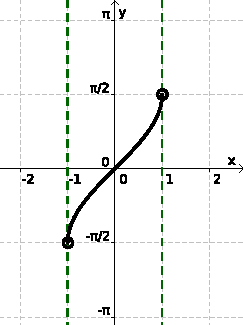
\includegraphics[width=5cm]{../Topicos/Figuras/arcsen.pdf}}
    \caption{Gráfico da função $f(x)= arcsen(x)$}
  \end{figure}
  

  \item Função Arco Cosseno: $f: [-1, 1] \rightarrow [0, \pi]$ dada por $f(x)= arccos(x)$, que também denotamos por $cos^{-1}(x)= arccos (x)$, neste caso temos o seguinte gráfico:

  \begin{figure}[H]
  \centering
    \fbox{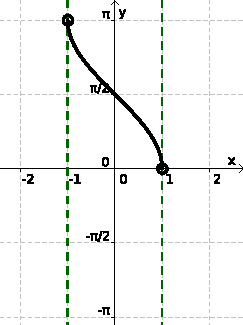
\includegraphics[width=5cm]{../Topicos/Figuras/arccos.pdf}}
    \caption{Gráfico da função $f(x)= arccos(x)$}
  \end{figure}
  
  
  \item Função Arco Tangente: $f: \R \rightarrow ]\frac{-\pi}{2}, \frac{\pi}{2}[$, dada por $f(x)= arctan(x)$ que também denotamos por $tan^{-1}(x)= arctan (x)$, neste caso o gráfico será:

  \begin{figure}[H]
  \centering
    \fbox{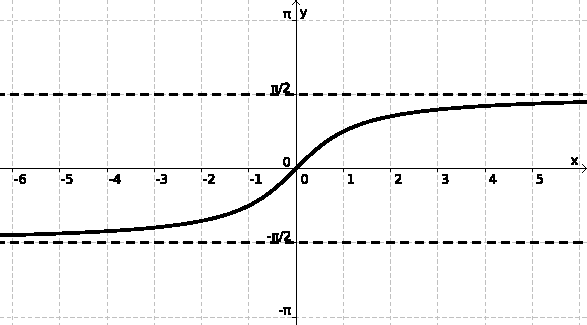
\includegraphics[width=10cm]{../Topicos/Figuras/arctan.pdf}}
    \caption{Gráfico da função $f(x)= arctan(x)$}
  \end{figure}
  

  \end{itemize}

  
  \newpage
 \section{Funções exponenciais}

  \colorbox{azul}{
 \begin{minipage}{0.9\linewidth}
 \begin{center}
 São funções $f: \R \rightarrow \R_{+}^{*} $ tais que:
 \[f(x) = a^x\]
 onde é dado $a \in \R_{+}$ satisfazendo $0 < a$ e $a \neq 1$. Estas funções são chamadas funções exponenciais de base $a$.
 \end{center}
 \end{minipage}}
 \vskip0.3cm
 
 Observe que:
 \begin{itemize}
  \item exigimos que a constante $a$ fosse positiva para garantir que a função estivesse definida para todo $x$ real (lembre-se que, por exemplo, $\sqrt{a}= a^{\frac{1}{2}}$ não está definida para $a$ negativo);
  \item excluímos $a=1$, pois $1^x=1$ para todo $x$ real, de modo que $f(x)= 1^x$ é uma função constante.
 \end{itemize}
 
 \begin{exem}\label{ex:exp-2}
  Considere a função $f: \R \rightarrow \R_{+}^{*} $ dada por, 
  \[f(x) = 2^x \ , \]
  vamos determinar alguns pontos do gráfico da função $f$.
 
  \begin{table}[H]
  \centering
  \begin{tabular}{|c|c|c|} \hline
  \rowcolor{cinza}
  $x$ & $f(x) = 2^x$ & $y$ \\ \hline
  $-2$ & $f(-2)= 2^{-2}= \dfrac{1}{2^2}$ & $\dfrac{1}{4}$ \\ \hline
  $-1$ & $f(-1)= 2^{-1}= \dfrac{1}{2^1}$ & $\dfrac{1}{2}$ \\ \hline
  $0$ & $f(0)= 2^{0}$ & $1$ \\ \hline
  $1$ & $f(1)= 2^{1}$ & $2$ \\ \hline
  $2$ & $f(2)= 2^{2}$ & $4$ \\ \hline
  \end{tabular}
  \end{table}
  
  Marcando estes pontos no plano cartesiano e ligando obtemos o seguinte gráfico para esta função.
  
  \begin{figure}[H]
  \centering
    \fbox{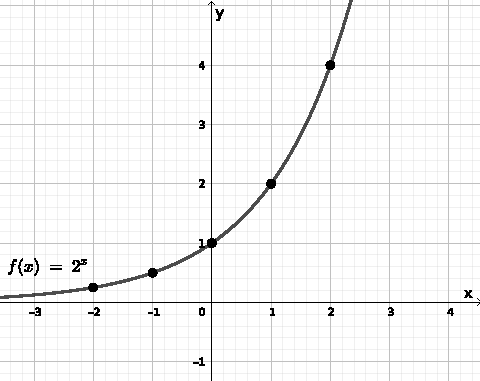
\includegraphics[width=7cm]{../Topicos/Figuras/f(x)=2^x.pdf}}
    \caption{Gráficos da função $f(x)=2^x$}
  \end{figure}
  
  Observe que neste caso a função é crescente, veremos que sempre que $1< a < +\infty$ a função exponencial $f(x)=a^x$ será crescente e seu gráfico será parecido com este.
 
 \end{exem}

 
  \begin{exem}\label{ex:exp-1/2}
  Considere a função $f: \R \rightarrow \R_{+}^{*} $ dada por, 
  \[f(x) = \left(\dfrac{1}{2}\right)^x \ , \]
  vamos determinar alguns pontos do gráfico da função $f$.
 
  \begin{table}[H]
  \centering
  \begin{tabular}{|c|c|c|} \hline
  \rowcolor{cinza}
  $x$ & $f(x) = \left(\dfrac{1}{2}\right)^x$ & $y$ \\ \hline
  $-2$ & $f(-2)= \left(\dfrac{1}{2}\right)^{-2}= 2^2$ & $4$ \\ \hline
  $-1$ & $f(-1)= \left(\dfrac{1}{2}\right)^{-1}= 2^1$ & $2$ \\ \hline
  $0$ & $f(0)= \left(\dfrac{1}{2}\right)^{0}$ & $1$ \\ \hline
  $1$ & $f(1)= \left(\dfrac{1}{2}\right)^{1}$ & $\dfrac{1}{2}$ \\ \hline
  $2$ & $f(2)= \left(\dfrac{1}{2}\right)^{2}$ & $\dfrac{1}{4}$ \\ \hline
  \end{tabular}
  \end{table}
  
  Marcando estes pontos no plano cartesiano e ligando obtemos o seguinte gráfico para esta função.
  
  \begin{figure}[H]
  \centering
    \fbox{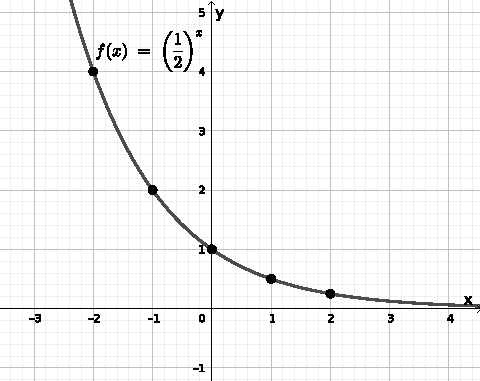
\includegraphics[width=7cm]{../Topicos/Figuras/f(x)=0_5^x.pdf}}
    \caption{Gráficos da função $f(x)=\left(\dfrac{1}{2}\right)^x$}
  \end{figure}
  
  Observe que neste caso a função é decrescente, veremos que sempre que $0< a < 1$ a função exponencial $f(x)=a^x$ será decrescente e seu gráfico será parecido com este.
 
 \end{exem}
 
 Para facilitar a comparação dos gráficos das funções dos dois últimos exemplos observe o plano cartesiano abaixo no qual temos os dois gráficos, note que eles são simétricos em relação ao eixo $y$.
 
   \begin{figure}[H]
 \centering
    \fbox{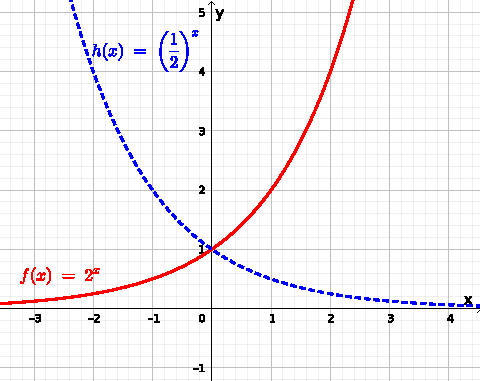
\includegraphics[width=8cm]{../Topicos/Figuras/comparandoexponenciais.pdf}}
    \caption{Comparando gráficos de funções exponenciais}
  \end{figure}


  \begin{exem} \label{ex:exp-e}
  Um caso especial de função exponencial é quando $a= e$, assim $f: \mathbb{R} \rightarrow \R_{+}^{*} $ será dada por:
  \[f(x) = e^x\]
  como $e= 2,7182818 \cdots$ decorre que $1 < e$ logo esta função é uma função crescente, e seu gráfico é:

  \begin{figure}[H]
 \centering
    \fbox{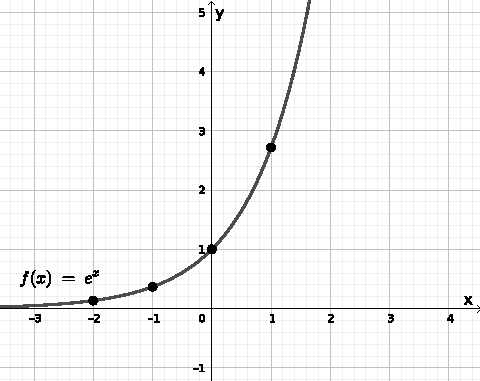
\includegraphics[width=7cm]{../Topicos/Figuras/f(x)=e^x.pdf}}
    \caption{Gráficos da função $f(x)= e^x$}
  \end{figure}
  \end{exem}

 \textbf{Propriedades:} Sejam $a, b \in \R_{+}^{*} \setminus \{1\}$ e $x, y \in \R$, nestas condições as seguintes propriedades são satisfeitas:
 \begin{enumerate}
  \item $a^x a^y= a^{x+y}$;
  \item $(a^x)^y= a^{xy}$;
  \item $(ab)^x= a^x b^x$;
  \item Se $0 < a < 1$ e $x < y$, então $a^x > a^y$, logo a função $f(x)= a^x$ é decrescente.
  \item Se $1 < a < +\infty$ e $x < y$, então $a^x > a^y$, logo a função $f(x)= a^x$ é crescente.
 \end{enumerate}
 
 De (4) obtemos que $f(x)= a^x$, $a > 1$, é estritamente crescente em $\R$. De (5) obtemos que $f(x)= a^x$, $0 < a < 1$, é estritamente decrescente em $\R$. Portanto $\forall a > 0$ e $a \neq 1$ temos que a função exponencial $f(x)= a^x$ é bijetora.
 
 Além destas são válidas aqui também todas as propriedades de potências que já são conhecidas do leitor.


 \section{Funções logarítmicas}

 \colorbox{azul}{
 \begin{minipage}{0.9\linewidth}
 \begin{center}
 São funções $f: \mathbb{R_{+}^{*}} \rightarrow \mathbb{R} $ tais que:
 \[f(x) = \log_{a}(x)\]
 onde é dado $a \in \mathbb{R}$ satisfazendo $0 < a$ e $a \neq 1$. Estas funções são denominadas funções logarítmicas de base $a$.
 \end{center}
 \end{minipage}}
 
 \vskip0.3cm
 

 Observemos que dado um número real $a> 0$ e $a \neq 1$, para cada $y>0$ existe um único número real $x$ tal que $a^x= y$, já que como visto anteriormente a função exponencial $f(x)= a^x$ é bijetiva. Podemos assim definir o logaritmo de $y$ na base $a$ como sendo o número real $x$ tal que $a^x= y$. Simbolicamente,
 \[\destaque{\log_a(y)= x  \Leftrightarrow a^x= y}.\]

 Portanto, as funções logarítmica e exponencial são inversas uma da outra.

 \begin{exem} \label{ex:log-2}
  Considere a função $h: \mathbb{R_{+}^{*}} \rightarrow \mathbb{R} $ tais que:
 \[h(x) = \log_{2}(x) \ .\]
 Vamos encontrar alguns pontos do gráfico da função $h$.
 
  \begin{table}[H]
 \centering
 \begin{tabular}{|c|c|c|c|} \hline
 \rowcolor{cinza}
 $x$ & $h(x) = \log_{2}(x)$ & $y$ \\ \hline
 $\dfrac{1}{8}$ & $h\left(\dfrac{1}{8}\right)= \log_{2}\left(\dfrac{1}{8}\right)$ & $-3$ \\ \hline
 $\dfrac{1}{4}$ & $h\left(\dfrac{1}{4}\right)= \log_{2}\left(\dfrac{1}{4}\right)$ & $-2$ \\ \hline
 $\dfrac{1}{2}$ & $h\left(\dfrac{1}{2}\right)= \log_{2}\left(\dfrac{1}{2}\right)$ & $-1$ \\ \hline
 $1$ & $h(1)= \log_{2}(1)$ & $0$ \\ \hline
 $2$ & $h(2)= \log_{2}(2)$ & $1$ \\ \hline
 $4$ & $h(4)= \log_{2}(4)$ & $2$ \\ \hline
 $8$ & $h(8)= \log_{2}(8)$ & $3$ \\ \hline
 \end{tabular}
 \end{table}
 
 \[\log_{2}\left(\dfrac{1}{8}\right)= y \Leftrightarrow 2^y= \dfrac{1}{8} \Leftrightarrow 2^y= 2^{-3} \Leftrightarrow y=-3\]
 \[\log_{2}\left(\dfrac{1}{4}\right)= y \Leftrightarrow 2^y= \dfrac{1}{4} \Leftrightarrow 2^y= 2^{-2} \Leftrightarrow y=-2\]
 \[\log_{2}\left(\dfrac{1}{2}\right)= y \Leftrightarrow 2^y= \dfrac{1}{2} \Leftrightarrow 2^y= 2^{-1} \Leftrightarrow y=-1\]
 \[\log_{2}(1)= y \Leftrightarrow 2^y= 1 \Leftrightarrow 2^y= 2^0 \Leftrightarrow y=0\]
 \[\log_{2}(2)= y \Leftrightarrow 2^y= 2 \Leftrightarrow 2^y= 2^1 \Leftrightarrow y=1\]
 \[\log_{2}(4)= y \Leftrightarrow 2^y= 4 \Leftrightarrow 2^y= 2^2 \Leftrightarrow y=2\]
 \[\log_{2}(8)= y \Leftrightarrow 2^y= 8 \Leftrightarrow 2^y= 2^3 \Leftrightarrow y=3\]
 
 \begin{figure}[H]
    \centering
    \fbox{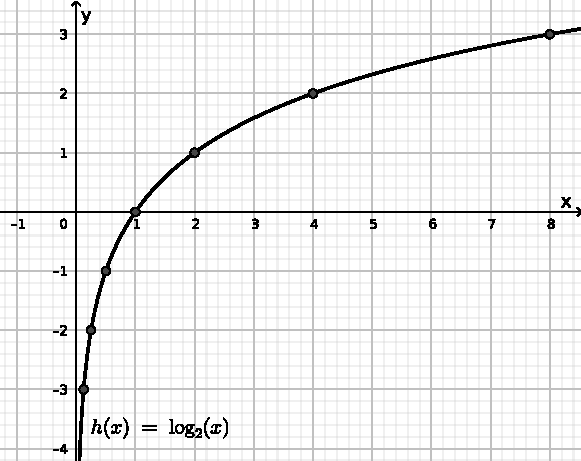
\includegraphics[width=7cm]{../Topicos/Figuras/h(x)=log_2.pdf}}
    \caption{Gráficos da função $h(x)= \log_{2}(x)$}
   \end{figure}
 Observe que a função $h(x)= \log_{2}(x)$ é estritamente crescente, veremos que sempre que $1< a < +\infty$ a função $h(x)= \log_{a}(x)$ será estritamente crescente e seu gráfico será parecido com este.
 \end{exem}

 \begin{exem} \label{ex:log-1/2}
    Considere a função $h: \mathbb{R_{+}^{*}} \rightarrow \mathbb{R} $ tais que:
 \[h(x) = \log_{\frac{1}{2}}(x) \ .\]
 Vamos encontrar alguns pontos do gráfico da função $h$.
 
  \begin{table}[H]
 \centering
 \begin{tabular}{|c|c|c|c|} \hline
 \rowcolor{cinza}
 $x$ & $h(x) = \log_{\frac{1}{2}}(x)$ & $y$ \\ \hline
 $\dfrac{1}{8}$ & $h\left(\dfrac{1}{8}\right)= \log_{\frac{1}{2}}\left(\dfrac{1}{8}\right)$ & $3$ \\ \hline
 $\dfrac{1}{4}$ & $h\left(\dfrac{1}{4}\right)= \log_{\frac{1}{2}}\left(\dfrac{1}{4}\right)$ & $2$ \\ \hline
 $\dfrac{1}{2}$ & $h\left(\dfrac{1}{2}\right)= \log_{\frac{1}{2}}\left(\dfrac{1}{2}\right)$ & $1$ \\ \hline
 $1$ & $h(1)= \log_{\frac{1}{2}}(1)$ & $0$ \\ \hline
 $2$ & $h(2)= \log_{\frac{1}{2}}(2)$ & $-1$ \\ \hline
 $4$ & $h(4)= \log_{\frac{1}{2}}(4)$ & $-2$ \\ \hline
 $8$ & $h(8)= \log_{\frac{1}{2}}(8)$ & $-3$ \\ \hline
 \end{tabular}
 \end{table}
 
 \[\log_{\frac{1}{2}}\left(\dfrac{1}{8}\right)= y \Leftrightarrow \left(\dfrac{1}{2}\right)^y= \dfrac{1}{8} \Leftrightarrow \left(\dfrac{1}{2}\right)^y= \left(\dfrac{1}{2}\right)^{3} \Leftrightarrow y=3\]
 
 
 \begin{figure}[H]
    \centering
    \fbox{\includegraphics[width=7cm]{../Topicos/Figuras/h(x)=log_12.pdf}}
    \caption{Gráficos da função $h(x)= \log_{1/2}(x)$}
   \end{figure}
 Observe que a função $h(x)= \log_{1/2}(x)$ é estritamente descrescente, veremos que sempre que $0< a< 1$ a função $h(x)= \log_{a}(x)$ será descrescente e seu gráfico será parecido com este.
 \end{exem}
 
 Para facilitar a comparação dos gráficos das funções dos dois últimos exemplos observe o plano cartesiano abaixo no qual temos os dois gráficos, note que eles são simétricos em relação ao eixo $x$.
 
   \begin{figure}[H]
 \centering
    \fbox{\includegraphics[width=8cm]{../Topicos/Figuras/comparandologs.pdf}}
    \caption{Comparando gráficos de funções logarítmicas}
  \end{figure}


  \begin{exem} \label{ex:log-e}
   Um caso especial de função logarítmica é quando $a= e$, assim $h: \mathbb{R_{+}^{*}} \rightarrow \mathbb{R} $ será dada por:
    \[h(x) = \log_{e}(x)= \ln(x)\]
  esta função é chamada logaritmo neperiano, que é uma função crescente, e seu gráfico é:

   \begin{figure}[H]
    \centering
    \fbox{\includegraphics[width=7cm]{../Topicos/Figuras/f(x)=ln(x).pdf}}
    \caption{Gráficos da função $h(x)= \ln(x)$}
   \end{figure}
   
 \end{exem}

  \textbf{Propriedades:} Sejam $a, b \in \R_{+}^{*} \setminus \{1\}$, e $k$ uma constante real qualquer. Se $x, y \in \R_{+}^{*}$, então:
  
  \begin{enumerate}
  \item $\log_{a}(a)= 1$;
  \item $\log_{a}(1)= 0$;
   \item $\log_{a}(x \cdot y)=\log_{a}(x) + \log_{a}(y)$;
   \item $\log_{a} \left(\frac{x}{y}\right)=\log_{a}(x) - \log_{a}(y)$;
   \item $\log_{a}(x^{k})= k \log_{a}(x)$;
   \item $\log_{a}(a^n)= n$;
   \item (Mudança de base) \[\log_{a}(x)=\frac{\log_{b}(x)}{\log_{b}(a)};\]
   \item Se $0 < a < 1$ e $x < y$, então $\log_{a}(x) > \log_{a}(y)$, logo a função $h(x)= \log_{a}(x)$ é descrescente;
   \item Se $a> 1$ e $x < y$, então $\log_{a}(x) < \log_{a}(y)$, logo a função $h(x)= \log_{a}(x)$ é crescente.
  \end{enumerate}
  
  Vamos agora demonstrar algumas destas propriedades.
  
  \textbf{Propriedade 1:} $\log_{a}(a)= 1$, note que:
  \[\log_{a}(a)= y \Leftrightarrow a^y = a \Leftrightarrow a^y= a^1 \Leftrightarrow y=1\]
  \fim
  
  \textbf{Propriedade 2:} $\log_{a}(1)= 0$, note que:
  \[\log_{a}(1)= y \Leftrightarrow a^y= 1 \Leftrightarrow a^y= a^0 \Leftrightarrow y=0\]
  \fim
    
  \textbf{Propriedade 3:} $\log_{a}(x \cdot y)=\log_{a}(x) + \log_{a}(y)$, para tal definimos:
  \begin{eqnarray*}
   a^b= x & \Leftrightarrow & b= \log_{a}(x) \\
   a^c= y & \Leftrightarrow & c= \log_{a}(y) \\
   a^{b+c}= z & \Leftrightarrow & b+c= \log_{a}(z)
  \end{eqnarray*}
  com isso obtemos que 
  \[x \cdot y= a^b \cdot a^c= a^{b+c}= z\]
  portanto,
  \[b+c= \log_{a}(z) \Rightarrow \log_{a}(x) + \log_{a}(y)= \log_{a}(x \cdot y)\]
  \fim
  
  \textbf{Propriedade 4:} $\log_{a} \left(\frac{x}{y}\right)=\log_{a}(x) - \log_{a}(y)$, para tal definimos:
  \begin{eqnarray*}
   a^b= x & \Leftrightarrow & b= \log_{a}(x) \\
   a^c= y & \Leftrightarrow & c= \log_{a}(y) \\
   a^{b-c}= z & \Leftrightarrow & b-c= \log_{a}(z)
  \end{eqnarray*}
  com isso obtemos que 
  \[\dfrac{x}{y}= \dfrac{a^b}{a^c}= a^{b-c}= z\]
  portanto,
  \[b-c= \log_{a}(z) \Rightarrow \log_{a}(x) - \log_{a}(y)= \log_{a}\left(\frac{x}{y}\right)\]
  \fim
  
  \textbf{Propriedade 5:} $\log_{a}(x^k)= k \log_{a}(x)$, note que,
  \[\log_{a}(x^k)= \log_{a}\underbrace{(x \cdot x \cdots x)}_{k-vezes}= \underbrace{log_{a}(x) + log_{a}(x)+ \cdots + log_{a}(x)}_{k-vezes}= k \cdot log_{a}(x)\]
  \fim
  
  \textbf{Propriedade 6:} $\log_{a}(a^n)= n$, note que:
  \[\log_{a}(a^n)= n \cdot \log_{a}(a)= n \cdot 1 = n\]
  \fim
  
  Anteriormente comentamos que a função exponencial de base $a$ tem como inversa a função logarítimo de base $a$, vamos agora retomar os exemplos que fizemos acima, para comparar os gráficos das exponenciais com seus repectivos logarítmos inversos. Vamos com isso observar que em todos os casos os gráficos são simétricos em relação ao gráfico da função identidade $Id(x)= x$.
  
  \begin{enumerate}
   \item Considere os exemplos \autoref{ex:exp-2} e \autoref{ex:log-2}, nestes exemplos apresentamos as funções $f(x)= 2^x$ e $h(x)= \log_{2}(x)$ respectivamente, cujos gráficos são simétricos em relação ao gráfico da função $Id$, como pode ser visto na figura abaixo, isso ocorre pois as funções $f$ e $h$ são inversas uma da outra.
   
   \begin{figure}[H]
    \centering
    \fbox{\includegraphics[width=9cm]{../Topicos/Figuras/comparandobase2.pdf}}
    \caption{Gráficos das funções exp e log de base $2$}
   \end{figure}
   
   \item Considere os exemplos \autoref{ex:exp-1/2} e \autoref{ex:log-1/2}, nestes exemplos apresentamos as funções $f(x)= \left(\frac{1}{2}\right)^x$ e $h(x)= \log_{\frac{1}{2}}(x)$ respectivamente, cujos gráficos são simétricos em relação ao gráfico da função $Id$, como pode ser visto na figura abaixo, isso ocorre pois as funções $f$ e $h$ são inversas uma da outra.
   
   \begin{figure}[H]
    \centering
    \fbox{\includegraphics[width=9cm]{../Topicos/Figuras/comparandobase1-2.pdf}}
    \caption{Gráficos das funções exp e log de base $\frac{1}{2}$}
   \end{figure}
   
   \item Considere os exemplos \autoref{ex:exp-e} e \autoref{ex:log-e}, nestes exemplos apresentamos as funções $f(x)= e^x$ e $h(x)= \ln(x)$ respectivamente, cujos gráficos são simétricos em relação ao gráfico da função $Id$, como pode ser visto na figura abaixo, isso ocorre pois as funções $f$ e $h$ são inversas uma da outra.
   
   \begin{figure}[H]
    \centering
    \fbox{\includegraphics[width=9cm]{../Topicos/Figuras/comparandobase-e.pdf}}
    \caption{Gráficos das funções exp e log de base $e$}
   \end{figure}
   
  \end{enumerate}


  
  
  

 \newpage
